%\documentclass[11pt]{article}
%\usepackage{graphicx}
%% This file is to hold any special settings for a particular CDR
% Things that are generic to CDRs in general go in cdr.cls.
% Probably no \usepackages should be here.

%\usepackage[pdftex,pdfpagelabels,bookmarks]{hyperref}



% This holds definitions of macros to enforce consistency in names.

% This file is the sole location for such definitions.  Check here to
% learn what there is and add new ones only here.  

% also see units.tex for units.

%%% Common terms

% Check here first, don't reinvent existing ones, add any novel ones.
% Use \xspace.

\def\expshort{LBN\xspace}
\def\explong{The Neutrino Experiment\xspace}

\def\anxlbnefd{Annex 4A: The LBNE Design for a Deep Underground Single-Phase Liquid Argon Time Projection Chamber\xspace}

% Things about oscillation
%
% example: \dm{12}
\newcommand{\dm}[1]{$\delta m^2_{#1}$\xspace}
% example \sinstt{12}
\newcommand{\sinstt}[1]{$\sin^22\theta_{#1}$\xspace}
% example \deltacp
\newcommand{\deltacp}{$\delta_{\rm CP}$\xspace}
% example \nuxtonux{\mu}{e}
\newcommand{\nuxtonux}[2]{$\nu_{#1} \to \nu_{#2}$\xspace}
\newcommand{\numutonumu}{\nuxtonux{\mu}{\mu}}
\newcommand{\numutonue}{\nuxtonux{\mu}{e}}
\newcommand{\numu}{$\nu_\mu$\xspace}
\newcommand{\nue}{$\nu_e$\xspace}
\newcommand{\anumu}{$\bar\nu_\mu$\xspace}
\newcommand{\anue}{$\bar\nu_e$\xspace}

% Names
\newcommand{\cherenkov}{Cherenkov\xspace}
\newcommand{\kamland}{KamLAND\xspace}
\newcommand{\kamiokande}{Kamiokande\xspace}
\newcommand{\superk}{Super--Kamiokande\xspace}
\newcommand{\miniboone}{MiniBooNE\xspace}
\newcommand{\minerva}{MINER$\nu$A\xspace}
\newcommand{\nova}{NO$\nu$A\xspace}
\newcommand{\SURF}{Sanford Underground Research Facility\xspace}


% This holds definitions of macros to enforce consistency in units.

% This file is the sole location for such definitions.  Check here to
% learn what there is and add new ones only here.  

% also see defs.tex for names.


% see
%  http://ctan.org/pkg/siunitx
%  http://mirrors.ctan.org/macros/latex/contrib/siunitx/siunitx.pdf

% Examples:
%  % angles
%  \ang{1.5} off-axis
%
%  % just a unit
%  \si{\kilo\tonne}
%
%  % with a value:
%  \SI{10}{\mega\electronvolt}

%  range of values:
% \SIrange{60}{120}{\GeV}

% some shorthand notation
\DeclareSIUnit \kton {\kilo\tonne}
\DeclareSIUnit \kt {\kilo\tonne}
\DeclareSIUnit \Mt {\mega\tonne}
\DeclareSIUnit \eV {\electronvolt}
\DeclareSIUnit \keV {\kilo\electronvolt}
\DeclareSIUnit \MeV {\mega\electronvolt}
\DeclareSIUnit \GeV {\giga\electronvolt}
\DeclareSIUnit \km {\kilo\meter}
\DeclareSIUnit \kW {\kilo\watt}
\DeclareSIUnit \MW {\mega\watt}
\DeclareSIUnit \MHz {\mega\hertz}
\DeclareSIUnit \mrad {\milli\radian}
\DeclareSIUnit \year {year}
\DeclareSIUnit \POT {POT}
\DeclareSIUnit \sig {$\sigma$}
\DeclareSIUnit\parsec{pc}
\DeclareSIUnit\lightyear{ly}
\DeclareSIUnit\foot{ft}
\DeclareSIUnit\ft{ft}
% for a bare kt-year
\def\ktyr{\si[inter-unit-product=\ensuremath{{}\cdot{}}]{\kt\year}\xspace}
\def\Mtyr{\si[inter-unit-product=\ensuremath{{}\cdot{}}]{\Mt\year}\xspace}
\def\msr{\si[inter-unit-product=\ensuremath{{}\cdot{}}]{\meter\steradian}\xspace}

\newcommand{\SIadj}[2]{\SI[number-unit-product = -]{#1}{#2}}
% Adjective form of some common units
% "the 10-kt detector"
\newcommand{\ktadj}[1]{\SIadj{#1}{\kt}}
% "the 1,300-km baseline"
\newcommand{\kmadj}[1]{\SIadj{#1}{\km}}
% "a 567-keV endpoint"
\newcommand{\keVadj}[1]{\SIadj{#1}{\keV}}
% "Typical 20-MeV event"
\newcommand{\MeVadj}[1]{\SIadj{#1}{\MeV}}
% "Typical 2-GeV event"
\newcommand{\GeVadj}[1]{\SIadj{#1}{\GeV}}
% "the 1.2-MW beam"
\newcommand{\MWadj}[1]{\SIadj{#1}{\MW}}
% "the 700-kW beam"
\newcommand{\kWadj}[1]{\SIadj{#1}{\kW}}
% "the 100-tonne beam"
\newcommand{\tonneadj}[1]{\SIadj{#1}{\tonne}}
% "the 4,850-foot depth beam"
\newcommand{\ftadj}[1]{\SIadj{#1}{\ft}}
%

% Mass exposure, people like to put dots between the units
% \newcommand{\ktyr}[1]{\SI[inter-unit-product=\ensuremath{{}\cdot{}}]{#1}{\kt\year}}
% must make usage of \ktyr above consistent with this one before turning on

% Beam x mass exposure, people like to put dots between the units
\newcommand{\ktmwyr}[1]{\SI[inter-unit-product=\ensuremath{{}\cdot{}}]{#1}{\kt\MW\year}}



% Set the major title, consistently across all volumes
\renewcommand\thevolumetitle{Conceptual Design Report \\ \explong}

% Do this here to make use of the experiment name and title macro
\hypersetup{
    pdftitle={\expshort CDR \thevolumesubtitle},
    pdfauthor={\expshort Collaboration},
    final=true,
    colorlinks=false,
    linktocpage=true,
    linkbordercolor=blue,
    citebordercolor=green,
    urlbordercolor=magenta,
    filecolor=black,
    pdfpagemode=UseOutlines,
    pdfborderstyle={/S/U},  
}




%\begin{document}
\chapter{Detector Development Program}
\label{ch:randd}

%\setlength{\parskip}{0.05in}

\section{Introduction}
This chapter describes the development program designed to ensure a successful and cost-effective construction and operation of the massive, dual-cryostat LArTPC detector for LBNE and to investigate possibilities for enhancing the performance of the detector. The feasibility of the LArTPC as a detector has been demonstrated most impressively by the  ICARUS experiment.
%current state of the ICARUS experiment currently taking data at Gran Sasso. (Anne rmvd 3/12)

It is understood that for successful operation an LArTPC has stringent requirements on
\begin{itemize}
 \item argon purity which must be of order 200~ppt O$_2$ equivalent or better
 \item long-term reliability of components located within the liquid argon; in particular, the TPC and field cage must be robust against wire-breakage and must support a cool-down of over 200~K
 \item the front-end electronics which must achieve a noise level ENC of $1000 e$ or better
\end{itemize}

The design of the LBNE LArTPC has evolved significantly from earlier concepts based on standard, above-ground, upright cylindrical LNG storage tanks which envisioned single TPC sense and high-voltage planes spanning the full width of the tank -- essentially a direct scaling of previous detectors. Problems with the actual construction of such massive planes and with the logistics of being able to construct the TPC only after the cryostat was complete are avoided in the present design. In our design,  TPC `panels'  are fully assembled and tested  --- including the electronics ---  independently of the cryostat construction. This modular approach is a key feature of the design. It has the benefit not only of improving the logistics of detector construction, but also the individual components can be of manageable size. It should also be noted that the cryostat itself is formed of modular panels designed for quick and convenient assembly.

\section{Components of the Development Program}
\label{sec:comp-dev-prog}

\fixme{This section needs review}

Programs of ongoing and planned development to allow the construction of massive LArTPCs in the U.S. have been developed and described in the {\em Integrated Plan for LArTPC Neutrino Detectors in the US}~\cite{IP}.
To advance the technology to the detectors proposed for LBNE, the U.S. program has three aspects:
\begin{itemize}
  \item a demonstration that the U.S program can reproduce the essential elements of the existing technology of the ICARUS program 
  \item a program of development on individual elements to improve the technology and/or 
         make it more cost-effective
  \item a program of development on how to apply the technology to a detector module
 \end{itemize}
 
A summary of the items in the program is given in the following tables. Table~\ref{tab:on-project} lists the activities that are part of the LBNE Project (``on-project'') described in this chapter, a short description of the information needed and the LBNE milestone corresponding to when the information is required. Table~\ref{tab:off-project} lists off-project activities, the aspect of these activities that is applicable to LAr-FD and the LBNE milestone at which the information is required. These aspects will be described in more detail in the following sections. As will be explained below, these are not R\&D activities, but rather elements of the preliminary engineering design process. 


\begin{cdrtable}[LBNE on-project development activities]{lp{4cm}p{4cm}}{on-project}{LBNE on-project development activities}
Activity & LAr-FD Information & Need by \\ \toprowrule
In-liquid Electronics & Low noise readout, long lifetime & CERN prototype construction \\ \colhline
TPC Construction & Mechanical design & CERN prototype construction\\ \colhline
35-ton Prototype & Cryostat construction & CERN prototype cryostat procurement \\ \colhline
CERN prototype & detector integration & TPC construction \\ 
\end{cdrtable}


\begin{cdrtable}[LBNE off-project development activities]{p{3cm}llp{2.5cm}}{off-project}
{LBNE off-project development activities}
Activity & LAr-FD Applicability & Status & Need by \\ \toprowrule
Yale TPC & None & Completed  & NA \\ \colhline
Materials Test System & Define requirements & Completed & NA \\
                              & Materials testing & Operating & As Req'd \\ \colhline
Electronics Test Stand & Electronics testing & Operating & As Req'd \\ \colhline
LAPD & Purity w/o evac. & Operating & LBNE CD2 \\ 
        & Convective flow  & Operating &  LBNE CD2 \\ \colhline
Scintillator Development & Photon Det. Definition & Completed & CERN prototype Construction \\ 
                                   & Industrialization &  Not started & LBNE CD3 \\ \colhline
ArgoNeuT   & Analysis tools   &   On-going & LBNE CD2 \\ \colhline
MicroBooNE & Electronics tests & Construction & LBNE CD3 \\ 
                  & DAQ algorithms &  In development & LBNE CD3 \\
                  & Analysis tools    &  In development & LBNE CD2 \\
                  & Lessons learned & Not started & LBNE CD3\\ 
\end{cdrtable}


%\section{Scope and Status of Individual Components}  Anne removed this 3/12/15 because too segmented

\section{Materials Test System}
\label{sec:mts}

\fixme{Do we need to say how old the MTS is?}

An area for LAr detector development, shown in Figure~\ref{fig:PAB}, has been established in the Proton Assembly Building at Fermilab. The Materials Test System (MTS) has been developed to determine the effect on electron-drift lifetime of materials and components that are candidates for 
inclusion in LAr-FD. The system essentially consists 
of a source of clean argon ($<30$ ppt O$_{2}$ equivalent), a cryostat, a sample chamber that can be purged or evacuated,  a mechanism for transferring a sample from the sample chamber into the cryostat, a mechanism for setting the sample height in the cryostat so that it can be placed either in the liquid or in the gas ullage above the liquid, a temperature probe to measure the temperature of the sample, and an electron-lifetime monitor. The system is fully automated and the lifetime data are stored in a single database along with the state of the cryogenic system. 

\begin{cdrfigure}[Liquid argon area at the Proton Assembly Building at Fermilab]{PAB}{Liquid argon area at the Proton Assembly Building at Fermilab}
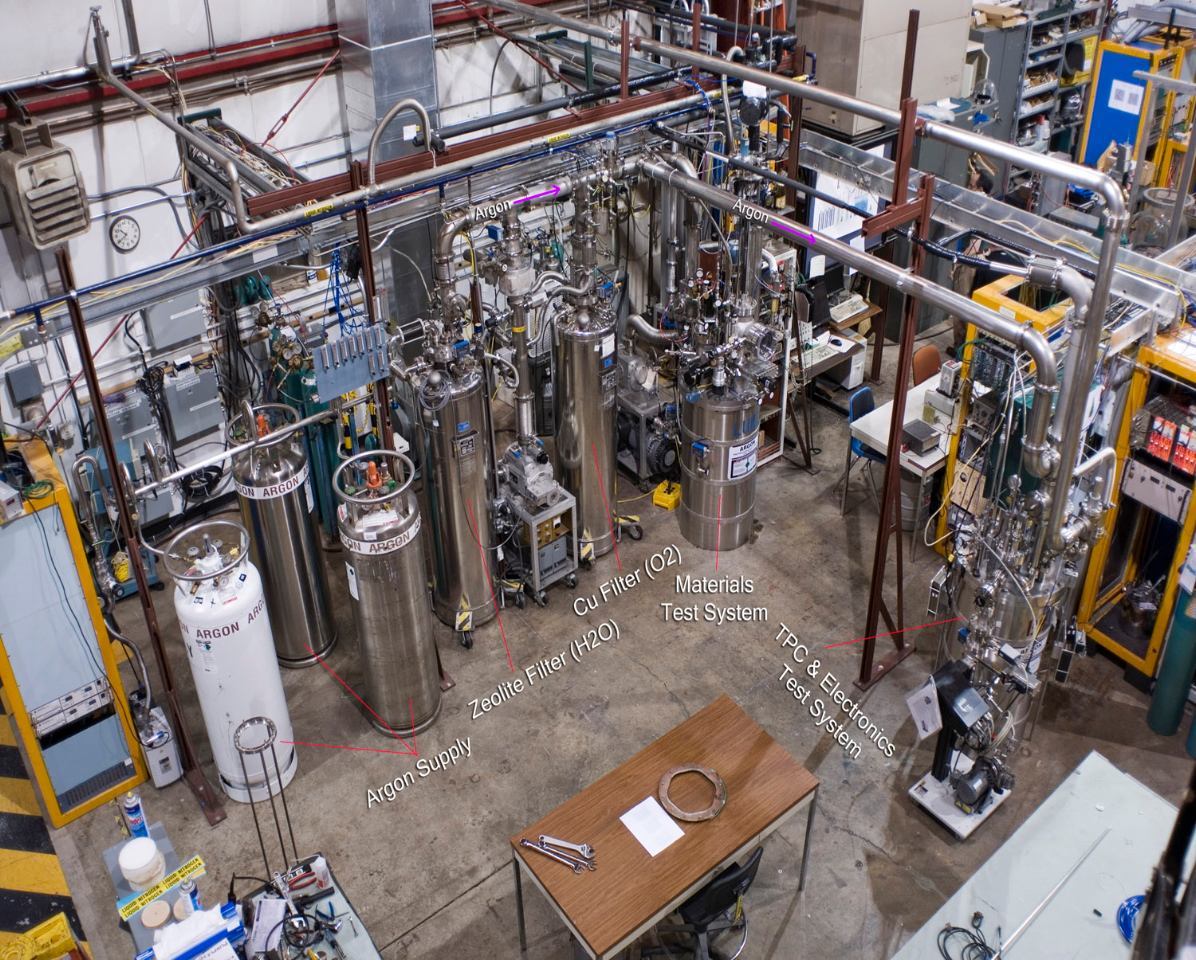
\includegraphics[width=0.8\textwidth]{LAratPAB.pdf}
\end{cdrfigure}
%

A noteworthy feature is the novel bubble-pump filter inside the cryostat. In case of argon contamination, this can filter the cryostat volume in a few hours, allowing us to continue studies %after the argon has been contaminated
 without having to refill. A schematic of the MTS is shown in Figure~\ref{fig:MTS_Schem}.

\begin{cdrfigure}[Schematic of the Materials Test System (MTS) cryostat at Fermilab]{MTS_Schem}{Schematic of the Materials Test System (MTS) cryostat at Fermilab}
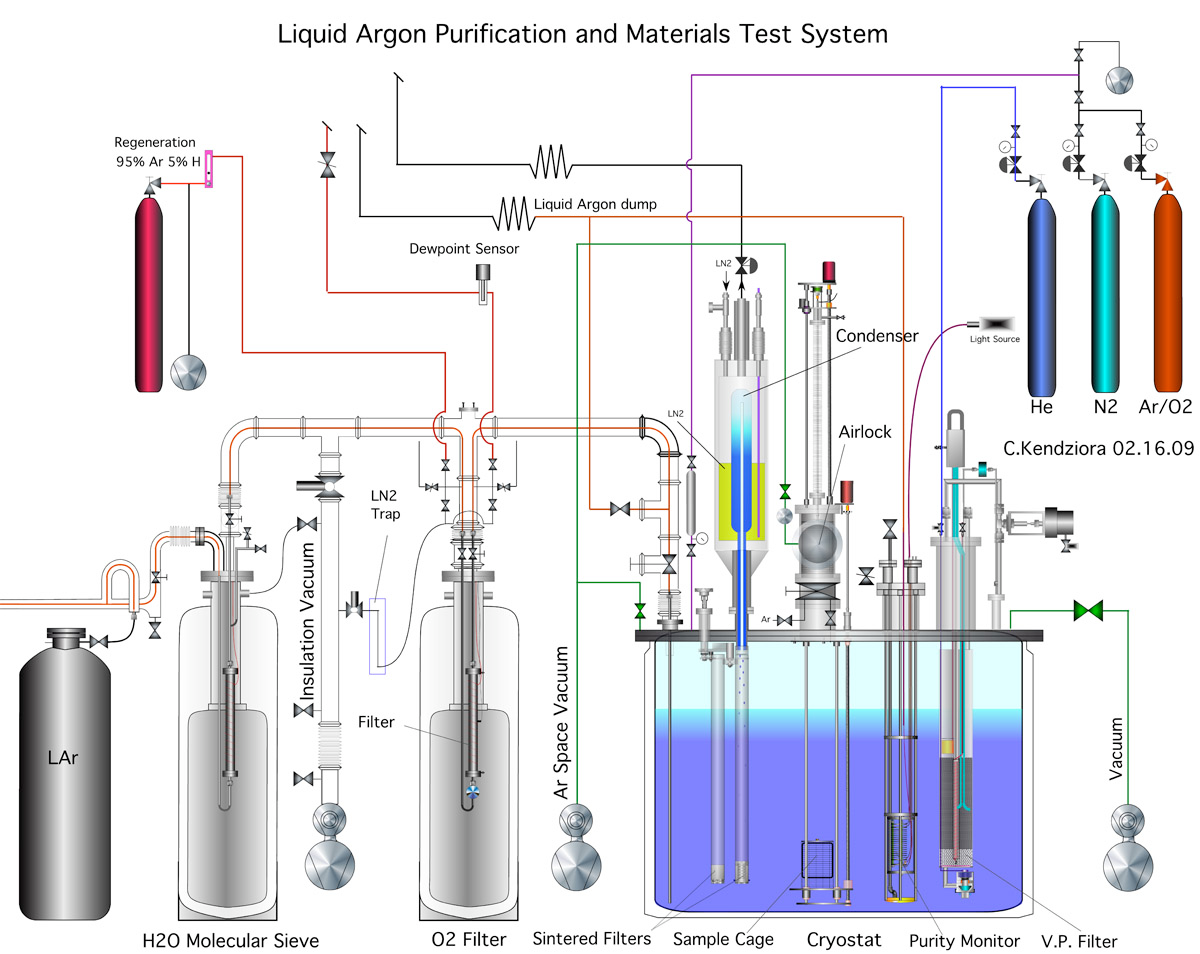
\includegraphics[width=0.9\textwidth]{MTS_Full_Schematic.pdf}
\end{cdrfigure}

The major conclusions of the studies to-date \fixme{today's to-date is different from when this was written} are summarized here. No material has been found that affects the electron-drift lifetime when the material is immersed in liquid argon -- this includes, for example, the common G-10 substitute, FR-4. On the other hand, materials in the ullage can contaminate the liquid; this contamination is dominated by the water outgassed by the materials and as a result is strongly temperature-dependent. Any convection currents that transport water-laden argon into the LAr and any cold surfaces on which water-laden argon can condense will fall into the LAr and reduce the electron lifetime. Conversely,  a steady flow of gaseous argon of a few ft/hr away from the LAr prevents any material in the gas volume from contaminating the LAr. 

These results are taken into account in the design of both MicroBooNE and LAr-FD. For LBNE they have been cast as detector requirements. The MTS will continue to be used by MicroBooNE and LBNE to test detector materials such as cables that will reside in the ullage.


\section{Photon Detection R\&D}

\fixme{Move to Photon chapter? Anne thinks the PD chapter already covers it.}

The R\&D program  for Photon Detection is based on a promising, new, cost-effective scheme for light collection in LArTPCs as described in a NIM article by Bugel et al~\cite{lightGuides}. The design is based upon lightguides fabricated from extruded or cast acrylic and coated with a wavelength-shifter doped skin.  Multiple acrylic bars are bent to guide light adiabatically to a single cryogenic PMT. Prototypes of the basic detector elements have been shown to perform well.  These lightguides have a thinner profile than the usual TPB-coated PMT-based system, occupying less space in an LAr vessel and resulting in more fiducial volume.  Another advantage of this system is that the bars are inexpensive to produce. The most convenient place for the paddles is between the wire planes that wrap around the APAs.

Lightguide R\&D has advanced rapidly since the initial publication resulting in $\sim$3 $\times$ higher light yields. The R\&D is now sufficiently advanced to provide a technical basis for the LAr-FD reference design. On-going design efforts at MIT, Indiana University, and Fermilab are directed toward industrial-scale production and the evaluation of lower-cost fluors that are effective in converting VUV photons. These efforts also include investigating PMTs with increased quantum efficiency as well as other efficient light-collection technologies, such as Geiger-mode avalanche photodiodes (commonly known as Silicon Photomultipliers, or SiPMs).

\subsection{TPC Design}
The design for LBNE has adopted the basic ICARUS multi-plane, single-phase TPC
concept and has incorporated new features suitable for a very large
detector.  The main emphasis of the development program is to develop a TPC design that is highly modular, low-cost, robust and easily installed inside a finished cryostat.

A significant effort has been focused on minimizing the dead space between detector modules to improve
the fiducial versus total LAr-volume ratio. The APA reference design accomplishes this goal but requires making $\sim$2 million high-quality wire terminations. The wire-termination scheme used by ICARUS has proven to be very reliable but it is too labor-intensive to fabricate for a million-channel detector system. We have adopted the wire-solder + wire-epoxy termination scheme that has been used for decades on drift chambers and proportional wire chambers to mount Cu-Be wires. The termination scheme was used to terminate 2.5 million  anode wires in the CMS end-cap muon system. Cu-Be wires have excellent mechanical properties and the advantage of low resistance compared to stainless steel. A study is currently underway within the LAr-FD subproject to identify the optimum wire-bonding parameters. The focus is currently on finding a commercial epoxy that optimizes the qualities of bond strength, cure time and low-temperature operation.

 \section{Electronics Development}
 \fixme{Mark C asks: remove, or move to Electronics section?}
 
 The work to-date on cold electronics has established that no show-stoppers exist. The remaining activities outlined here concern performance optimization of the CMOS ASICs, the evaluation of several widely available CMOS technologies, and the development of readout architectures appropriate and timely for various scenarios of very large detectors.

\subsection{CMOS Transistors: Lifetime Verification and Technology Evaluation}

The results of the design of the CMOS electronics for operation at LAr temperature (89~K), performed so far by the MicroBooNE and LBNE collaborations, as well as by a large collaboration led by Georgia Inst. of Technology, are summarized in Section~\ref{sec:v5-tpc-elec}.

Briefly, the fundamentals are: charge-carrier mobility in silicon increases at 89~K, thermal fluctuations decrease with kT/e, resulting in a higher gain (transconductance/current ratio =
 $g_{m}/ i$), higher speed and lower noise. For a given drain-current density the same degree of impact ionization (measured by the transistor substrate current) occurs at a somewhat lower drain-source voltage at 89~K than at 300~K. The charge trapped in the gate oxide and its interface with the channel causes degradation in the transconductance (gain) of the transistor and a threshold shift. The former is of major consequence as it limits the effective lifetime of the device (defined in industry and the literature as 10\% degradation in transconductance). Thus an MOS transistor has equal lifetime due to impact ionization at 89~K and at 300~K at different drain-source voltages. This is illustrated in Figure~\ref{fig:DSV}.  

This feature offers a tool for accelerated-lifetime testing by stressing the transistor with both increased current and increased voltage, and monitoring the substrate current and the change  in $g_{m}$ due to impact ionization. In these conditions, the lifetime can be reduced arbitrarily by many orders of magnitude, and the limiting operating conditions for a lifetime in excess of $\sim$20 years can be determined. With this foundation, more conservative design rules (lower current densities and voltages) can be derived and applied in the ASIC design, as has been done for the ASIC described in Section \ref{subsec:fe-arch}. The goal of this part of the program is to verify by accelerated testing the expected lifetimes for the several widely available CMOS technologies under consideration (TSMC, IBM, AMS). It should be noted that this is a standard test method used by the semiconductor industry. These methods are used to qualify electronics for deep space NASA missions as well as commerical PCs.
 
\begin{cdrfigure}[Lifetime at different temperatures vs V$_{DS}$]{DSV}{Lifetime at different temperatures vs V$_{DS}$}
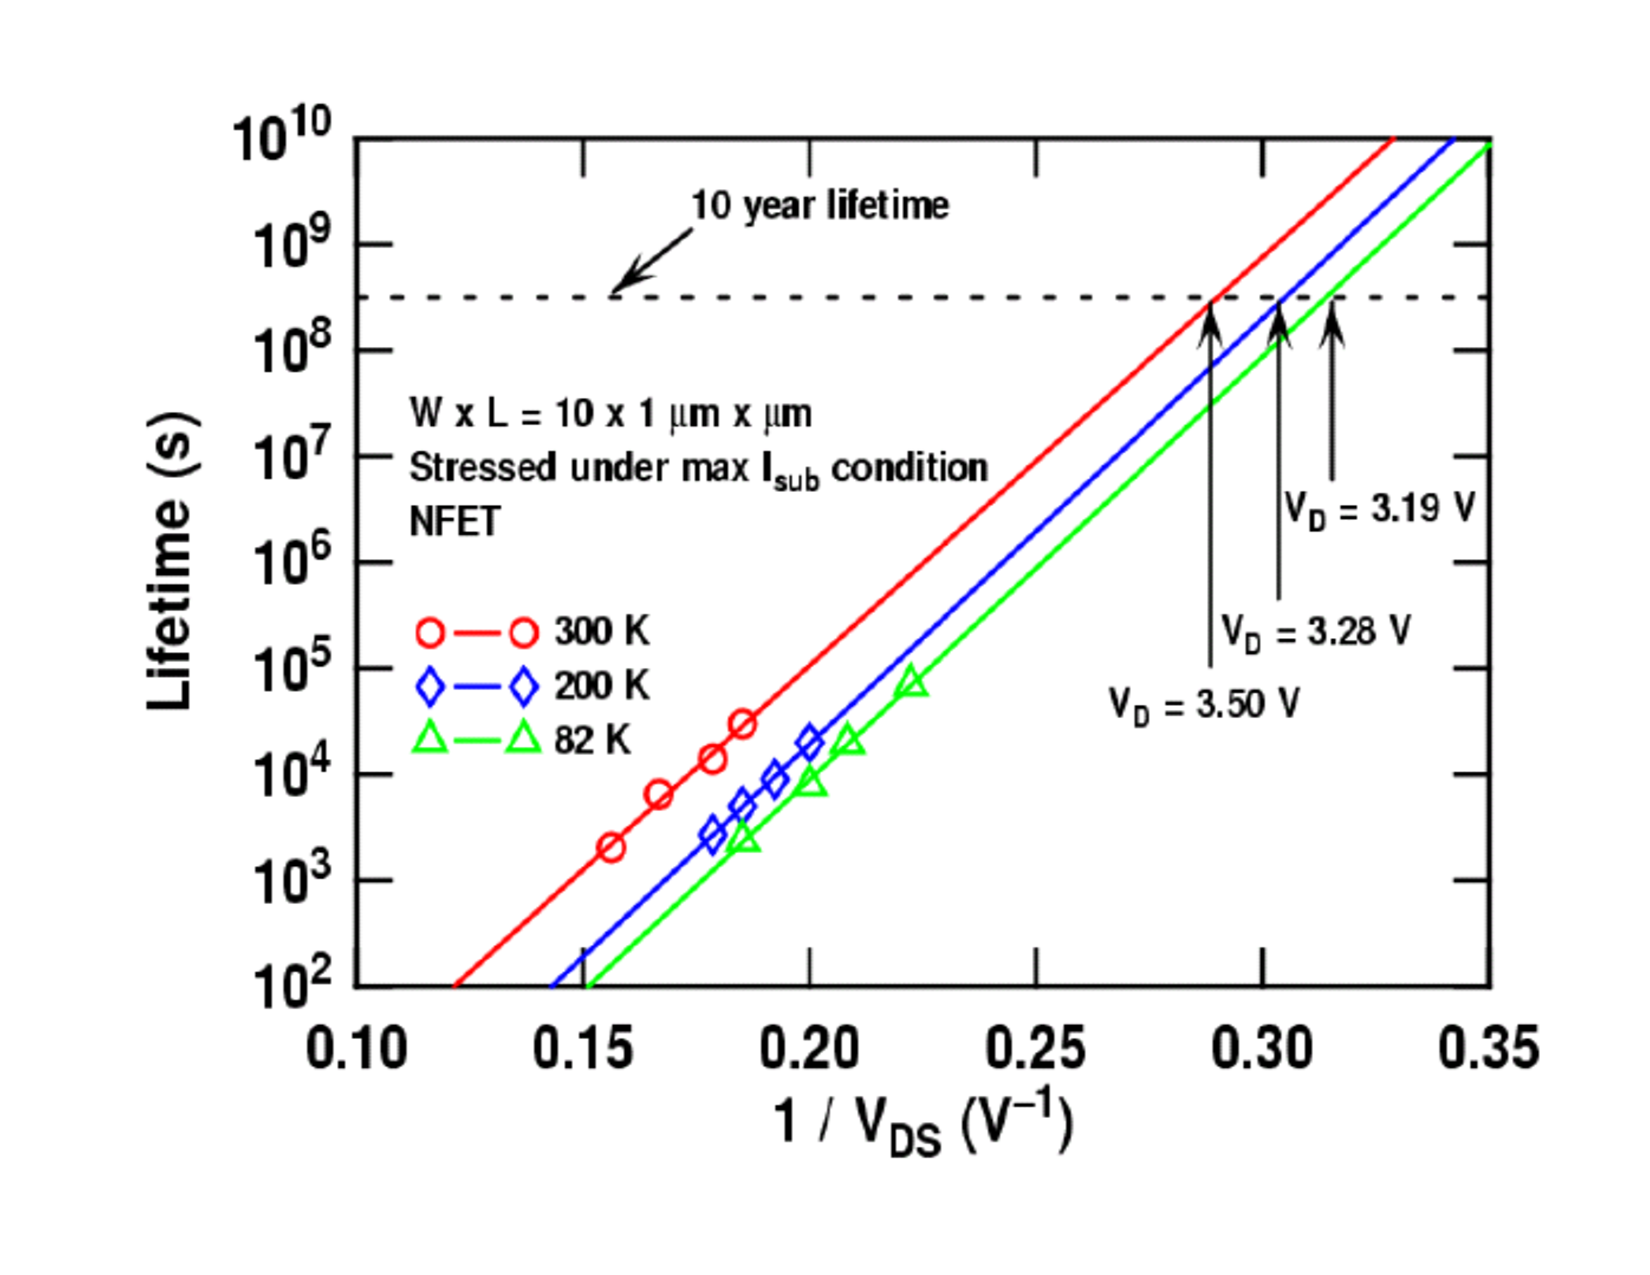
\includegraphics[width=0.75\textwidth]{LifetimetestVR}
\end{cdrfigure}

\subsection{Readout Architectures, Multiplexing and Redundancy}
A high degree of multiplexing after digitization of signals is essential for a TPC with 0.5 million wires in order to reduce the cable plant and the attendant outgassing. Just how high a multiplexing factor should be chosen is a matter of study, considering the risk of losing one output data link. A part of the
program will include system designs with redundant links and redundant final multiplexing stages to minimize the risk of losing the data from a significant fraction of the TPC (note that even with a multiplexing factor of 1/1024 and no redundancy, one failed link would result in a loss of 0.2\%).


\section{35-ton Prototype}
\fixme{Need explanation of phase 1 vs 2}

\subsection{Phase 1 Cryostat Development}
\label{35tonprototype}
\fixme{This is out of date}

The next step in the cryostat-prototype program is intended to address project-related issues: (1) to gain detailed construction experience, (2) to develop the procurement and contracting model for LAr-FD and (3) to incorporate the design and approval mechanism in the Fermilab ES\&H manual. (Membrane cryostats are designed in accordance with European and Japanese standards.) At present, we are in the process of procuring the cryostat components for a 35-ton membrane cryostat from IHI.

The LBNE project has contracted with the Japanese company IHI to build a small prototype membrane cryostat at Fermilab.  This approximately 35-ton unit is to be built and made operational in 2012 at Fermilab's PC-4 facility where LAPD is located.  It is intended to demonstrate high-purity operation in this type of cryostat and the suitability of the planned LAr-FD construction techniques and materials.  The testing programs for LAPD and the small prototype will be similar.  LBNE's 35-ton membrane cryostat will use a large portion of the cryogenic-process equipment installed for LAPD.

\begin{cdrfigure}[Layout of 35-ton prototype at Fermilab's PC-4 facility]{v5ch2-35ton-2011}{Layout of 35-ton prototype at Fermilab's PC-4 facility}
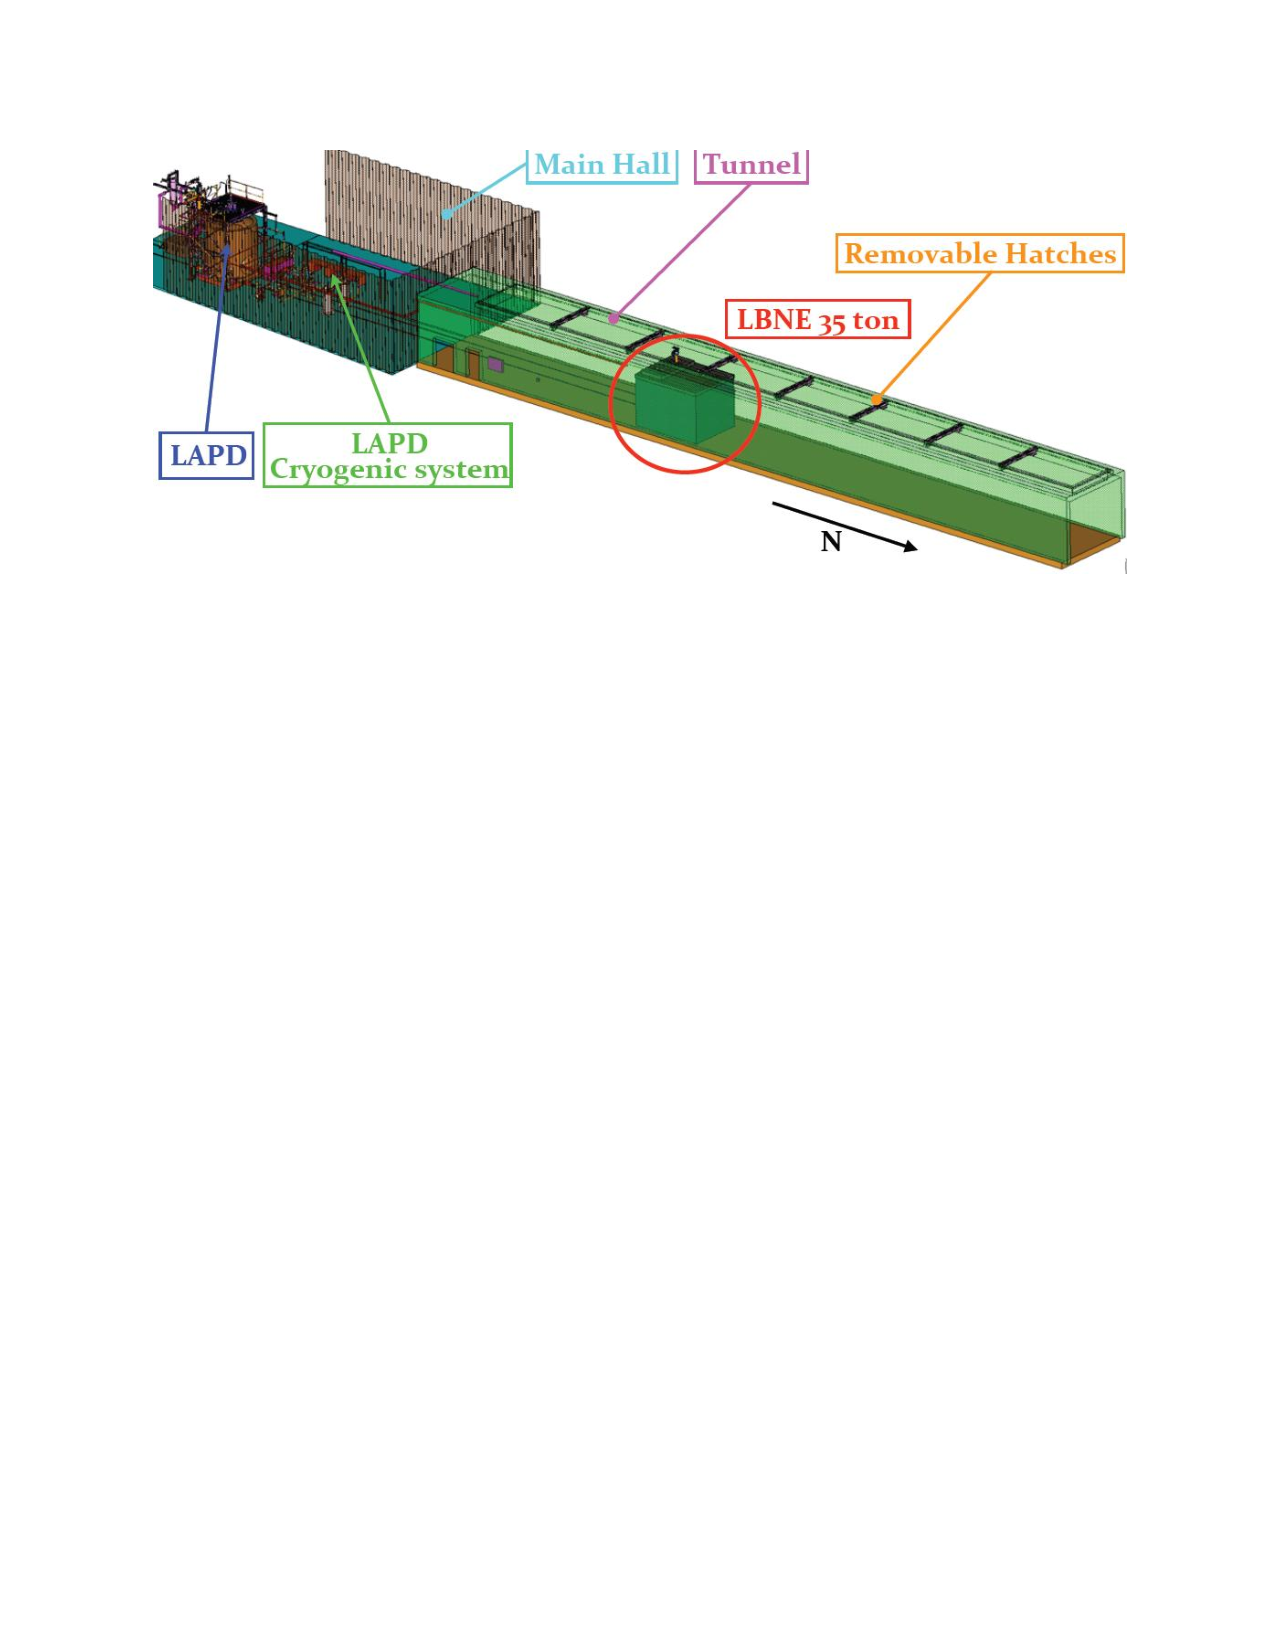
\includegraphics[width=\textwidth]{v5ch2-35ton-2011} 
\end{cdrfigure}

The prototype membrane cryostat's total size, including insulation and concrete support, is approximately 4.1~m $\times$ 4.1~m $\times$5.4~m, and will hold approximately 826~tons of LAr. The insulation thickness will be 0.4~m rather than the 1.0~m chosen for our reference design.  The techniques of membrane-cryostat construction will be demonstrated to be a fit for high-purity TPC service.  Welding of corrugated panels, removal of leak-checking dye penetrant or ammonia-activated leak-detecting paints, and post-construction-cleaning methods will be tested for suitability of service.  Residual contamination measurements at different elevations during the initial GAr purge process will be compared to computational predictions and will validate the purge-process modeling of a large rectangular vessel.  The prototype membrane cryostat will be filled with LAr.  Purity levels of the liquid with time and electron-drift times will be measured using purity monitors installed in the liquid bath.  Heat-load measurements will be made and compared to calculations. Eventually, connectors and feedthroughs, ports and other features that are planned for the reference design will be incorporated into the prototype.  Materials and cold-electronics testing can be done along with electron-drift-time measurements.

In principle, a thin-walled membrane cryostat is as suitable as a thick-walled cryostat for use with high purity LAr. Both would be constructed with 304 stainless steel with a polished surface finish. Both would use passive insulation. The total length of interior welds required for construction would be similar in both cases. The leak checking procedure would be the same in both cases.

The significant difference between membrane cryostats and thick-walled cryostats is the depth of the welds used to construct the vessel.  The majority of membrane-cryostat welds are completed in one or two passes with automatic welding machines. A second difference, and a major advantage, is that the membrane cryostat is a standard industrial design that has been in use for over 40 years. A thick-walled cryostat vessel would be custom designed and would require significant engineering and testing. A third difference, and another major advantage, is the ability to purge the membrane cryostat insulation space with argon gas so that a leak cannot affect the purity if it escapes detection and repair. 

A 3-m $\times$ 3-m wall panel shown in Figure~\ref{fig:3panel} was constructed at Fermilab using materials and technical guidance from GTT. The labor hours used in construction are consistent with the vendor estimates. The wall panel was leak tested (none were found) and vacuum tests were performed on the insulation system. We found that the insulation system is designed to allow vacuum pumping of the main cryostat volume to a hard vacuum. This result demonstrates that vacuum pumping of a membrane cryostat is feasible, if it is found to be required. No modifications to the vendor-supplied components are required to accomplish this.


\begin{cdrfigure}[Membrane panel assembly and components]{3panel}{Membrane panel assembly and components}
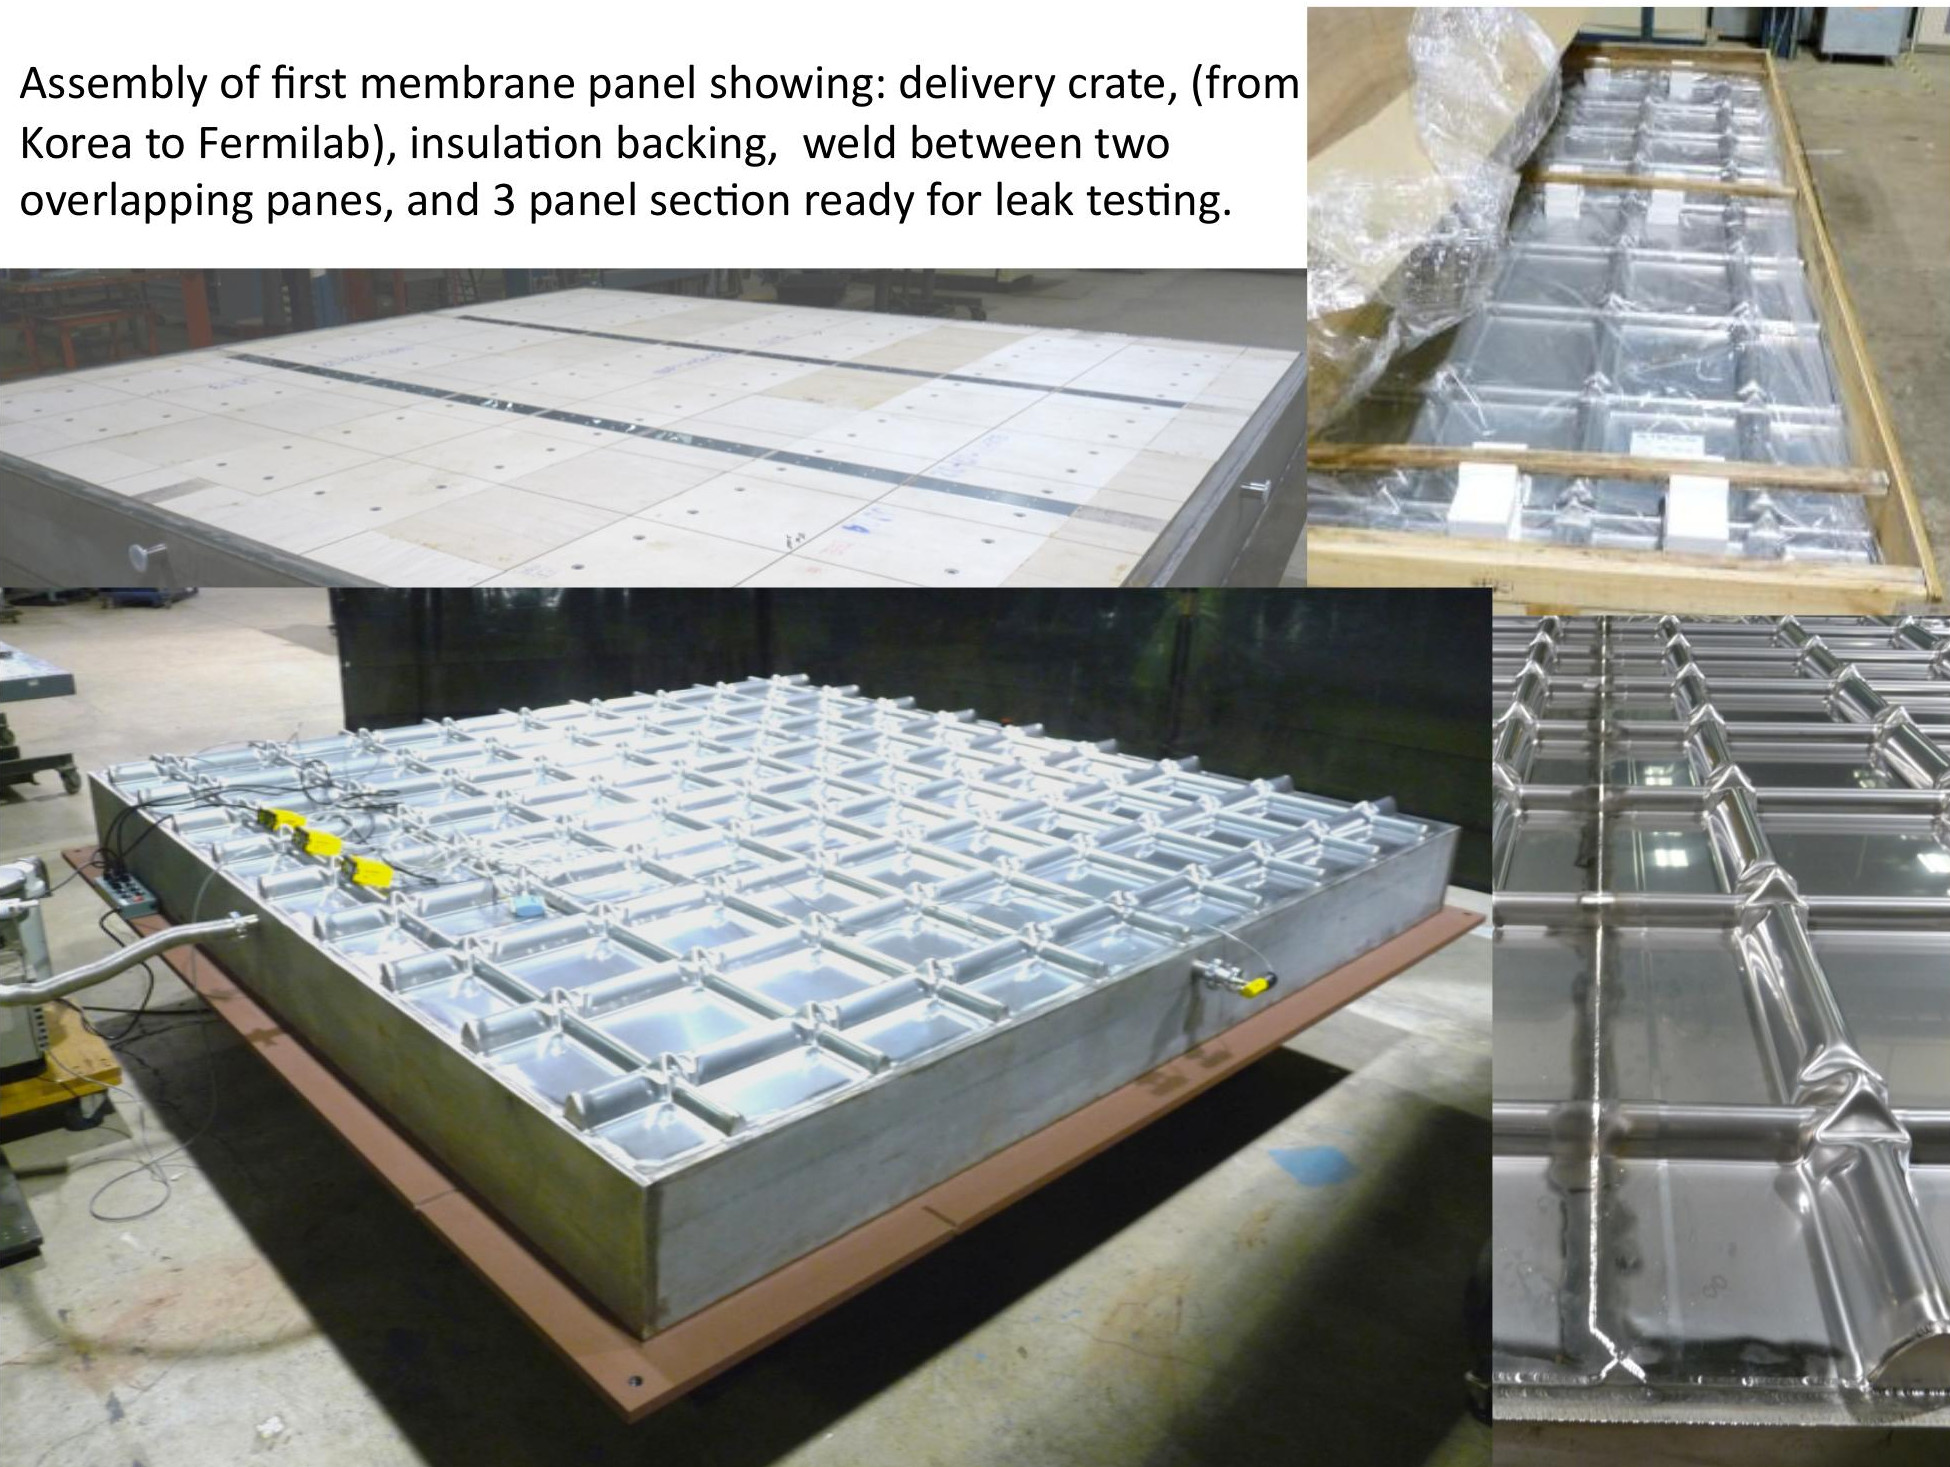
\includegraphics[width=0.7\textwidth]{Membranepastichepage}
\end{cdrfigure}

%%%%%%%%%%%%%%%%%%%%%%%%%%%%  from Alan Hahn Mar 11, 2015

\subsection{Phase 1 Test}

The 35-ton Prototype Cryostat (35T) is a small demonstration project to show the suitability of the 
membrane technology for LAr detectors. In particular that it can achieve and hold the needed purity 
levels and provide a stable environment for the TPC. A cutaway drawing of the 35T is shown in 
Figure~\ref{fig:cutaway}.


\begin{cdrfigure}[35T Cutaway Drawing.]{cutaway}{Cutaway drawing of the 35 Ton Cryostat showing construction details with exterior and interior dimensions.}
  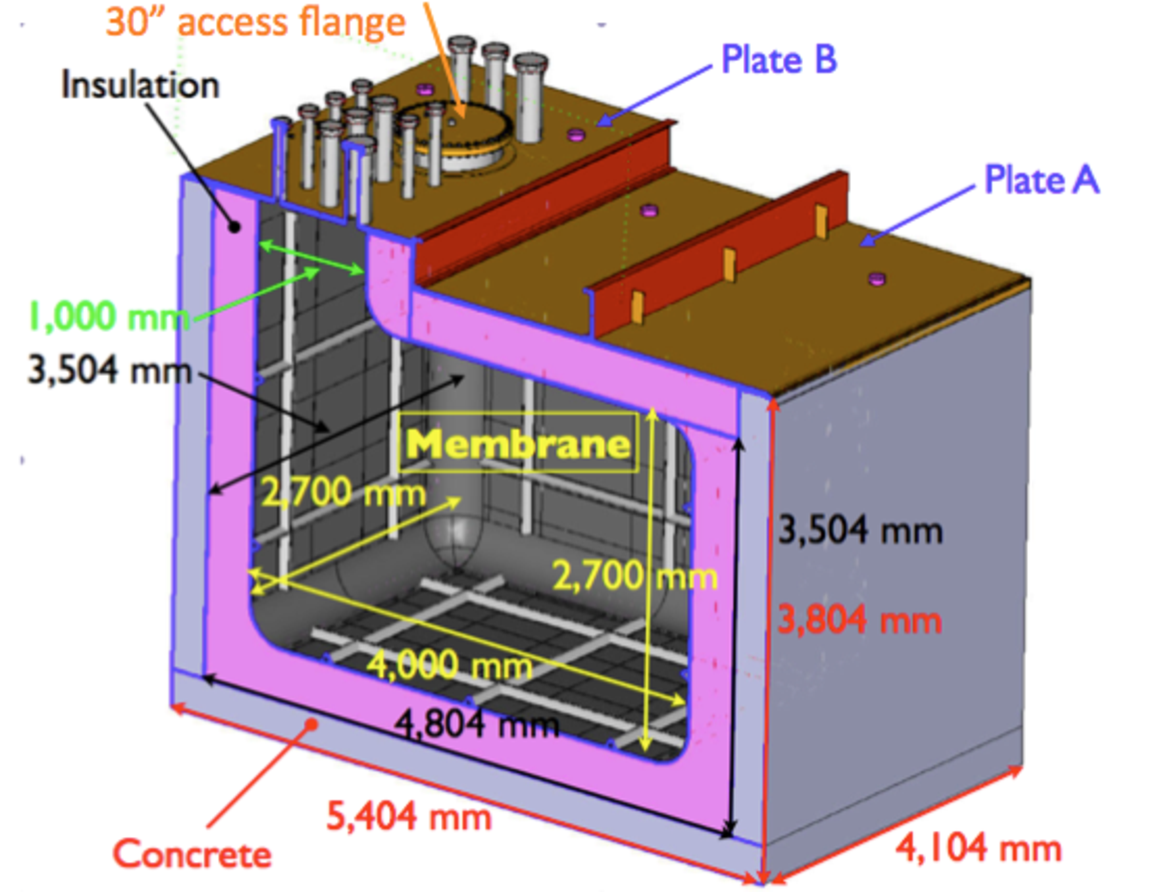
\includegraphics[width=0.8\textwidth]{35TCutaway}
\end{cdrfigure}

The 35T was constructed in 2012 in a decommissioned beam line (Proton Center) at Fermilab. This 
location is adjacent to another LAr cryostat, the Liquid Argon Purity Demonstrator (LAPD) [1].\fixme{}
 This 
enabled the 35T to reuse the existing purification and instrumentation infrastructure of LAPD (see 
Figure~\ref{fig:35TLayout}). The proximity and size (30 tons) of LAPD also offers the possibility using LAPD as 
a partial storage vessel for LAr if the 35T would need to be emptied. The 35T employs a submersible LAr 
pump to pump the LAr from the cryostat to the filters. Two pumps were installed for redundancy, but 
only one is used at a time.

\begin{cdrfigure}[35T Layout in PC4]{35TLayout}{Drawing of arrangement of the 35T and LAPD in Proton Center beam line.}
  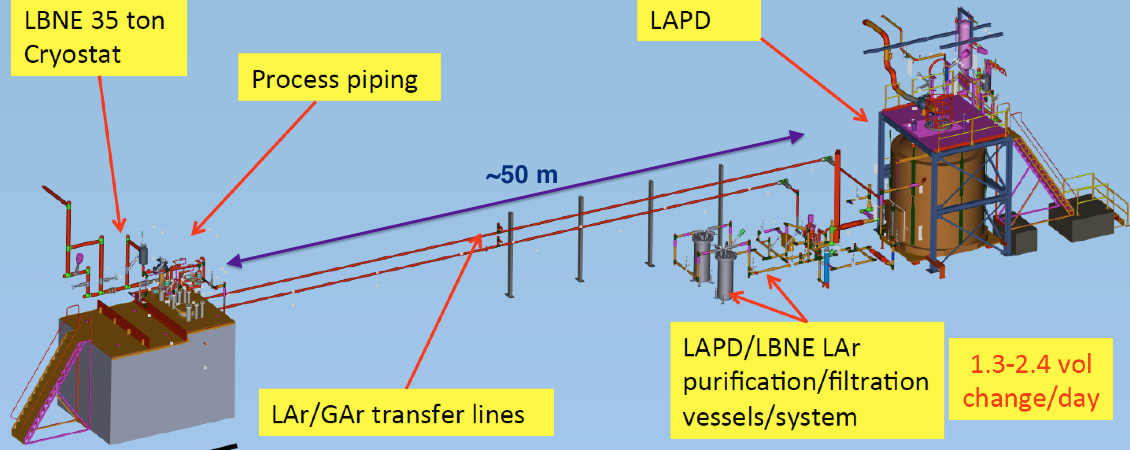
\includegraphics[width=1.0\textwidth]{35TLayout}
\end{cdrfigure}

Table~\ref{tab:35Tdimensions} gives the details of the construction materials and the dimensions for the 35T. More information can be found in [2].

\begin{cdrtable}[35T Details and Dimensions]{ll}{35Tdimensions}
{35T Details and Dimensions}
Parameter & Value \\ \toprowrule
Cryostat Volume	&      29.16 m3\\ \colhline
Liquid Argon total mass	 &     38.6 metric tons\\ \colhline
Inner dimensions	&      4.0 m (L) x 2.7 m (W) x 2.7 m (H)\\ \colhline
Membrane		&      2.0 mm thick corrugated 304 SS\\ \colhline
Insulation		&      0.4 m polyurethane foam\\ \colhline
Secondary barrier system	   &   0.1 mm thick fiberglass\\ \colhline
Vapor barrier	Normal	  &    1.2 mm thick carbon steel\\ \colhline
Steel reinforced concrete	    &  0.3 m thick layer\\ 
\end{cdrtable}

%%%%%%%%%%%%%%%%%%%%%%%%%%%%
\subsubsection {Phase 1 Instrumentation}

The 35T includes a full complement of standard commercial transducers and sensors that are used to 
monitor and control the cryogenic environment. They include temperature sensors, pressure transducers 
(absolute and gauge), flow meters, and level sensors. These devices are typically readout directly into the 
Control System and data logged. 

A number of commercial gas analyzers are available that can measure trace impurity levels (O$_2$, H$_2$O, and 
N$_2$) in the argon. Some have sensitivities at the 100 ppt level. A gas distribution switchyard feeding the 
gas analyzers allows the sampling points in the 35T to be reconfigured.

There were also two purpose-built pieces of instrumentation for the monitoring of the high-purity 
environment needed for a LAr detector. They are the purity monitors (PrMs) and the RTD Spooler. The 
PrMs are used to measure electron lifetimes in the LAr, and the RTD Spooler is used to make precision 
measurements of the temperature profile of the cryostat as a function of depth.  These instruments were 
originally constructed for the LAPD run and are described in depth in [1]\fixme{}.

%%%%%%%%%%%%%%%%%%%%%%%%%%%%
\subsubsection {Phase 1 Operations}

In order to purify LAr, it is necessary to do three things: 1) remove the air from the cryostat, leaving only Ar gas, 2) clean the liquid Ar as it comes from the supplier, and 3) remove any impurities that are generated by materials outgassing within the cryostat.  
LAPD has demonstrated that it is not necessary to evacuate a cryostat in order achieve LAr purity levels sufficient for LBNE. This is of paramount importance since the costs of multi-kiloton cryostats that could withstand evacuation is prohibitive. The 35T followed the procedure LAPD [1] established to obtain and maintain pure LAr. 

%%%%%%%%%%%%%%
\subsubsubsection {A. Gas Phase}

Figure~\ref{fig:35TPurge} graphically shows step 1, removing the ambient air, of the purification process. These measurements are made by a variety of gas monitors that are sampling the gas in the cryostat. 

\begin{cdrfigure}[Gas Ar Purge and Recirculation]{35TPurge}{Gas phase of removing impurities in the 35T. These quantities are being measured by various gas analyzers. The first stage of the purification is a process called the ``Piston Purge''.  The second stage is ``Recirculation with Filtering''. The gap between the two steps was due to troubleshooting a leak.}
  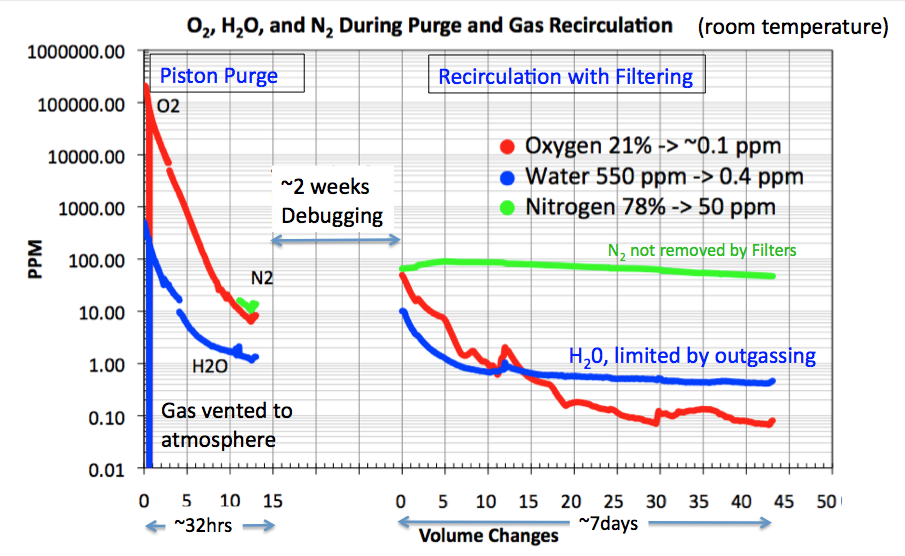
\includegraphics[width=\textwidth]{35TPurgeAndRecirc}
\end{cdrfigure}

The initial state of the 35T was that ``dry'' air had been purging the cryostat for approximately three weeks. The initial start values for oxygen, water, and nitrogen reflect this state.
The air in the cryostat is removed by  the Piston Purge.  Argon gas is flooded into the bottom of the cryostat. As argon is heavier than air, the argon layer rises analogous to a mechanical piston, pushing the air up and out of the cryostat. This gas is vented to the outside atmosphere. The venting stage continues for 32 hours, approximately the equivalent of 12 volume changes. 

At this point the exiting gas is re-routed to circulate through the filtration system that removes O$_2$ and H$_2$O. N$_2$ is not materially removed by the filters. Any leaks to the outside atmosphere can be detected during this step. As shown in Figure~\ref{fig:35TPurge}, a leak was found and mitigated (the ``Debugging'' gap in the plot). Once leaks have been eliminated the recirculation continues until the O$_2$ level drops into the sub-ppm level. As can be seen in the plot, the H$_2$O level plateaus at a much higher level than O$_2$. This is due to the outgassing of materials inside the 35T, including the cryostat walls, which are at room temperature during the recirculation step. 

%%%%%%%%%%%%%%
\subsubsubsection {B. Cool down and LAr filling}

\begin{cdrfigure}[35T Cooldown and Filling]{35TCooldown}{Cooldown and filling the 35T. The 
measurements (red trace) are made from RTDs afixed to the cryostat walls. The black dashed curve is the 
manufacturer's maximum allowed cooldown rate. The filling (blue trace) was from the transfer of LAr 
from LAPD, This quantity of LAr is less than the capacity of the 35T. The RTD traces drop to the LAr 
temperature when the level of the LAr covers reaches their mounting height.}
  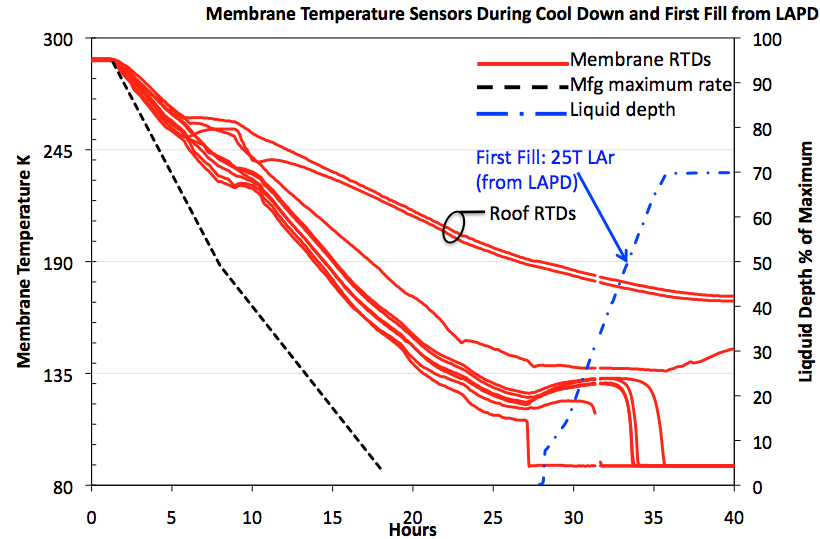
\includegraphics[width=\textwidth]{35TCoolDown.png}
\end{cdrfigure}

We have adopted a gas/liquid spray method to cool down the cryostat. This generates a turbulent mixing 
of cold gas in the cryostat and cools the entire surface. The cool down rate was limited to be less than 
the maximum rate specified by the membrane cryostat manufacturer. The cool down, as well as the initial 
filling is shown in Figure~\ref{fig:35TCooldown} . The temperature measurements (red traces) in this plot 
were made by RTDs that are glued to the membrane walls of the cryostat. The black dashed trace is the 
manufacturer specification for the cool down rate.

Once the cool down was finished, the LAr transfer into the cryostat began. In the case of the 35T phase 1 
run, the LAr came from LAPD, where it had been used by that system in its own recently completed 
second run [1]\fixme{}. 

LAPD contained about 30 tons of LAr, of which only 25 tons could be transferred to the 35T ($\sim$70\% of 
the total possible 35T LAr volume). It was decided that we would begin the initial commissioning of the 
Phase 1 run with this level since several components of the 35 Ton could be commissioned with the 
partial LAr fill. After running with this partial fill for approximately eighteen days, additional LAr was 
added to bring the capacity to 100\%. 

%%%%%%%%%%%%%%
\subsubsubsection{C. LAr Purification}

The Fermilab Material Test Stand (MTS) [4]\fixme{} has shown that contaminants released inside LAr filled cryostats are from materials outgassing in the warm ullage regions above the LAr surface. Typical detector materials located in LAr have negligible impact of LAr purity levels. 

Figure~\ref{fig:35TVaporFlow} depicts how impurities generated by outgassing materials in the 
relatively warm ullage under Plate B are swept up by the normal Ar boil-off in the 35T. This impure vapor 
is condensed in the LN2-cooled LAr condensor. The impure condensate is returned to the 35T just inside 
the intake manifold of the interior submersible LAr pump. From there it is pumped to the filtration 
system where the impurities are removed.

Of interest, the electron lifetime of the LAr exiting the filters, as measured by the inline PrM was always  
> 30 ms (purity ~ 10 ppt O2 equivalent). This indicates that the filters are very efficient at removing all 
trace amounts of O2 and H2O. This was true for the entire 35T phase 1 run, including the filling periods.

\begin{cdrfigure}[35T Vapor Flow]{35TVaporFlow}{Drawing of Boiloff/Outgassing Vapor Flow (white 
arrows) from the Cryostat, with condensate return (violet arrows) from the condensor into the Pump 
Intake Manifold. LAr flow into the pump, and return from the Purification filters are shown by blue 
arrows. Also shown is the location of the Stainless Steel Radiation baffles beneath Plate B. This location 
just beneath Plate B is the warmest location and presumably the principal source of outgassing within the 
cryostat.}
  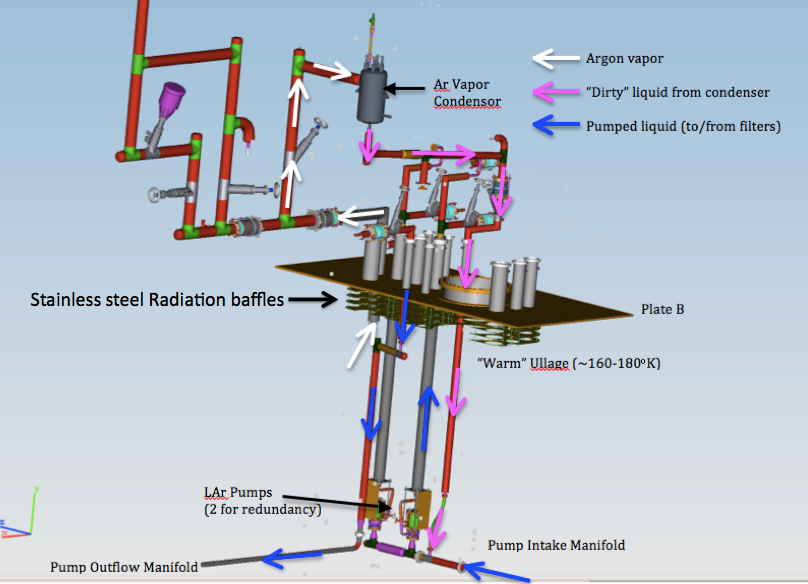
\includegraphics[width=\textwidth]{35TVaporFlow}
\end{cdrfigure}

Figure~\ref{fig:35TElectronLifetime} shows the electron lifetime from the start of the LAr Pump operation until the Phase 1 run ended. In general the electron lifetime improved as a function of pump on-time, but there were several incidents that spoiled the lifetime. These will be discussed in the next section.

%%%%%%%%%%%%%%%%%%%%%%%%%%%%
\subsubsection {Phase 1 Stability of Operation}

The goals of the 35T Phase 1 run include not only achieving the required purity/lifetime levels, but to 
also hold those levels and provide a stable operation of the cryostat. The 35T Phase 1 run was a relatively 
short  ~2 months of LAr running. We achieved electron lifetimes in the 2-3 ms range as can be seen in 
Figure~\ref{fig:35TElectronLifetime}.

However the electron lifetimes were severely impacted whenever we would switch from one LAr pump to 
another. The drops in purity coincided with the turn on of the previously-inactive pump (see annotations 
in Figure~\ref{fig:35TElectronLifetime}). We believe the issue was with the procedure we used to start the 
pumps and plan to modify it for future operations in the 35T Phase 2 run.

A second stability question is keeping the temperature stable in the cryostat. Currently the 35T controls 
system regulates the gauge pressure of the cryostat, keeping the internal pressure to 6.69(02) kPa above 
ambient atmospheric pressure. However this leaves the thermodynamics of the LAr sensitive to normal 
atmospheric pressure changes.

\begin{cdrfigure}[35T Electron Lifetime]{35TElectronLifetime}{LAr electron lifetmes as measured by 
Cryostat Purity Monitors. Significant events are annotated on the plot. Major divisions on horizontal axis 
are one week periods. Equivalent purity levels are shown as dashed horizontal lines.}
  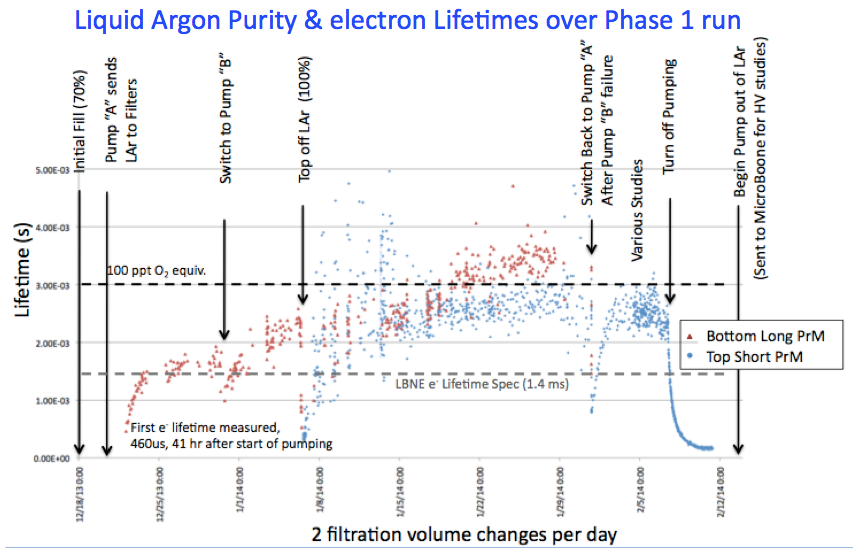
\includegraphics[width=0.8\textwidth]{35TElectronLifetime}
\end{cdrfigure}

Figure~\ref{fig:35TTempStability} is a plot over a nine day period of the Cryostat absolute pressure (blue 
trace), bulk LAr temperature (white dashed trace) and the normalized drift time of three PrMs, one short 
and long inside the cryostat, and the long inline PrM exterior to the cryostat. The temperature is taken 
from the RTD Spooler measurements by requiring that the RTDs be at least 15 cm below the LAr surface. 
The temperature curve lags the pressure changes ($\Delta P \sim~3.5$~kPa over this period), due to the thermal 
inertial of the LAr. However the normalized drift time (= drift time/(average drift time for this period) is 
directly correlated to the LAr temperature. The LAr temperature excursion range was $\Delta T \sim~0.3$~K. 
Fitting the normalized drift velocity (inverse of normalized drift time) gives the result 

% won't compile $\Delta_{\fract{driftspeed}{\overline{driftspeed}}} = -\fract{0.022}{001}~K$\\

 $\Delta_{driftspeed/\overline{driftspeed}} = -0.022/001~K$\\
 
The electron drift velocities for these three PrMs varied from (0.3 to 0.4) mm/$\mu$s depending on the individual PrM's drift field. 

\begin{cdrfigure}[35T Temperature Stability]{35TTempStability}{Interior Cryostat Absolute Pressure 
(blue trace), bulk LAr temperature (white dashed trace), and PrM drift times (dots) over a nine-day period. 
Major divisions on horizontal axis are one day intervals. The PrM drift times are from three PrMs, two in 
the cryostat, and the third from the inline PrM. The lag between the temperature and pressure is due to 
the 35T thermal inertia.}
  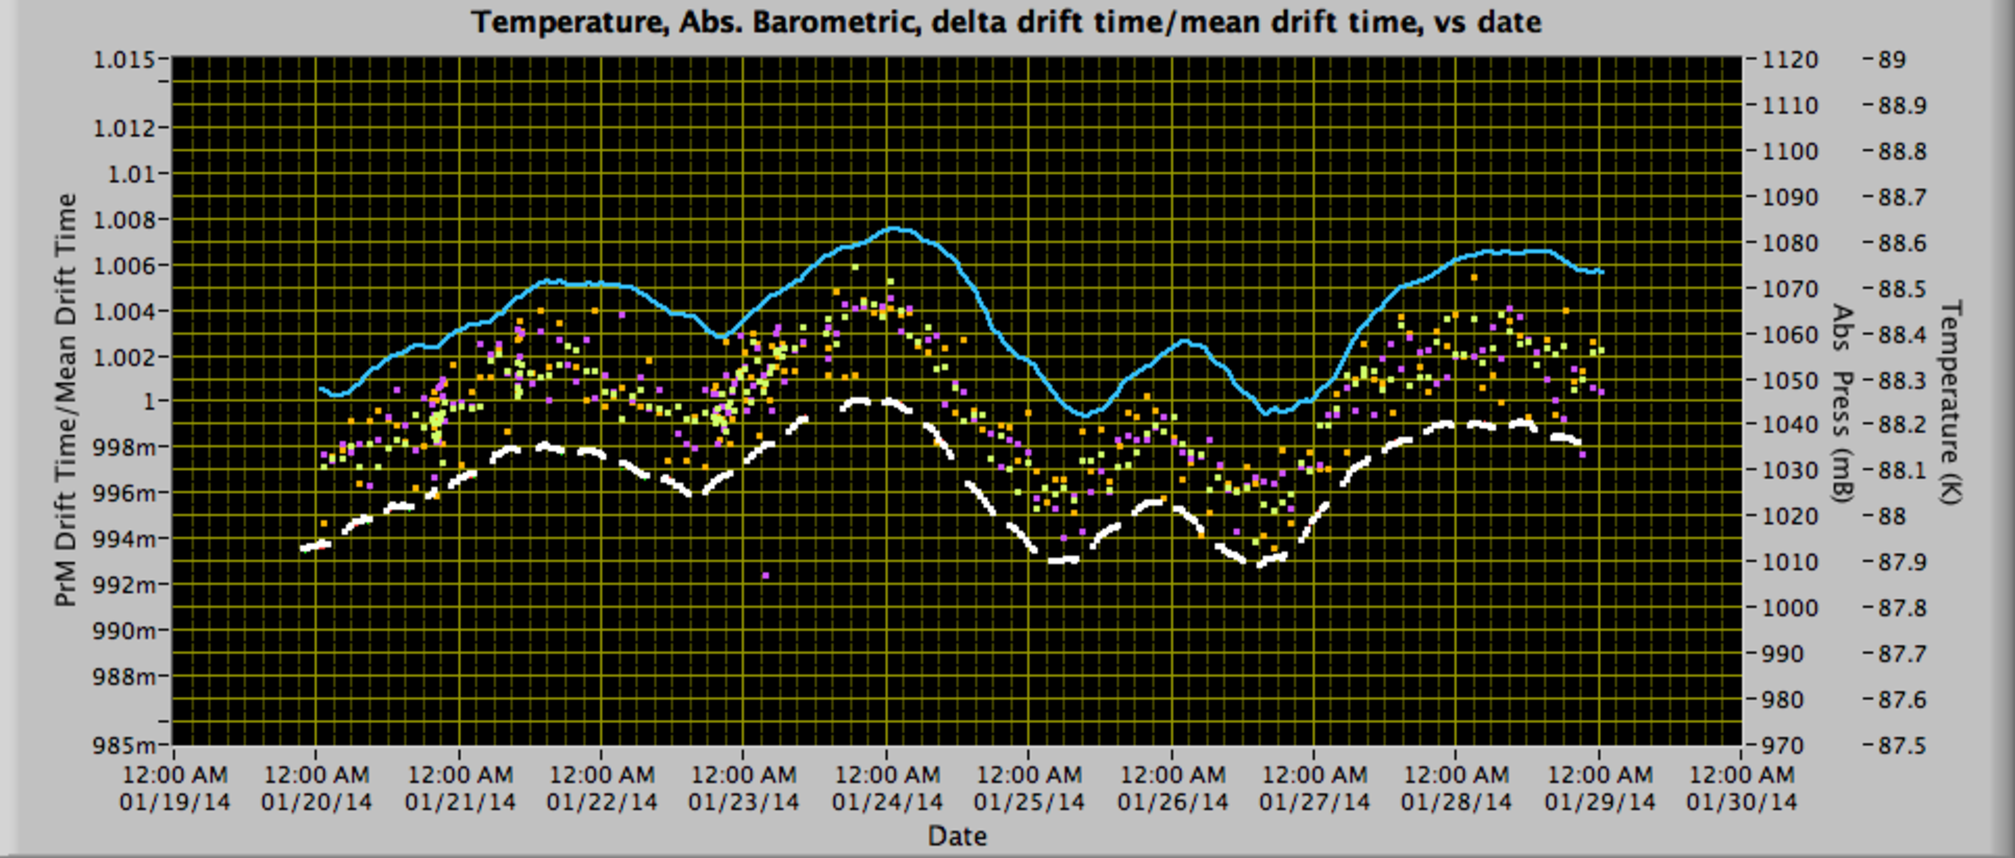
\includegraphics[width=\textwidth]{35TTempStability}
\end{cdrfigure}

The RTD Spooler was intended to give us a precision measurement of the vertical temperature profile. 
This measurement is a means of testing the Computational Fluid Dynamics Simulations [5]\fixme{} that 
are being made on the fluid motion in the cryostat. Experimentally measuring the actual motion does not 
appear to be feasible at this time. The CFD calculations are being used to understand whether there 
might be dead areas in the cryostat where impurities might collect. Figure~\ref{fig:SpoolerScan} shows the result of one RTD 
scan. This scan was taken from a period where the barometric pressure was relatively constant so that 
the temperature would remain constant during the scan. Since a scan takes up to 6 hours in one direction 
(up or down) and as can be seen in Figure~\ref{fig:35TTempStability}, pressure changes can impact the 
bulk temperature of the LAr. These profiles seen in Figure~\ref{fig:SpoolerScan} are in nominal 
agreement with the current CFD calculations [5\fixme{}].


\begin{cdrfigure}[35T Vertical Temperature Profile]{SpoolerScan}{(top) RTD Spooler Vertical Temperature scan of the 35T Cryostat under Plate B showing both the liquid and vapor temperature.  (bottom) Expanded horizontal axis around 88.12~K. Note that the horizontal divisions on the lower plot are 50~mK. }
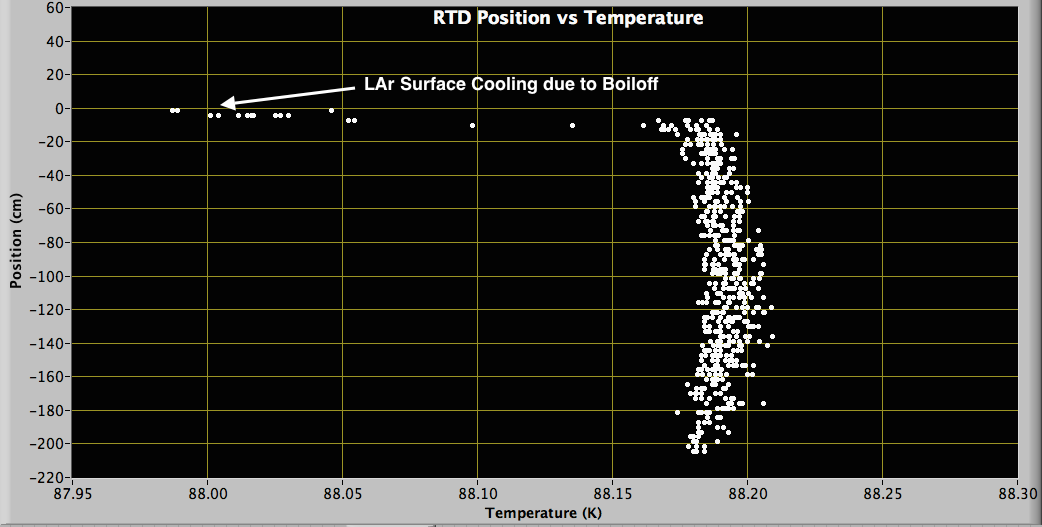
\includegraphics[width=\textwidth]{SpoolerScanExpand}  
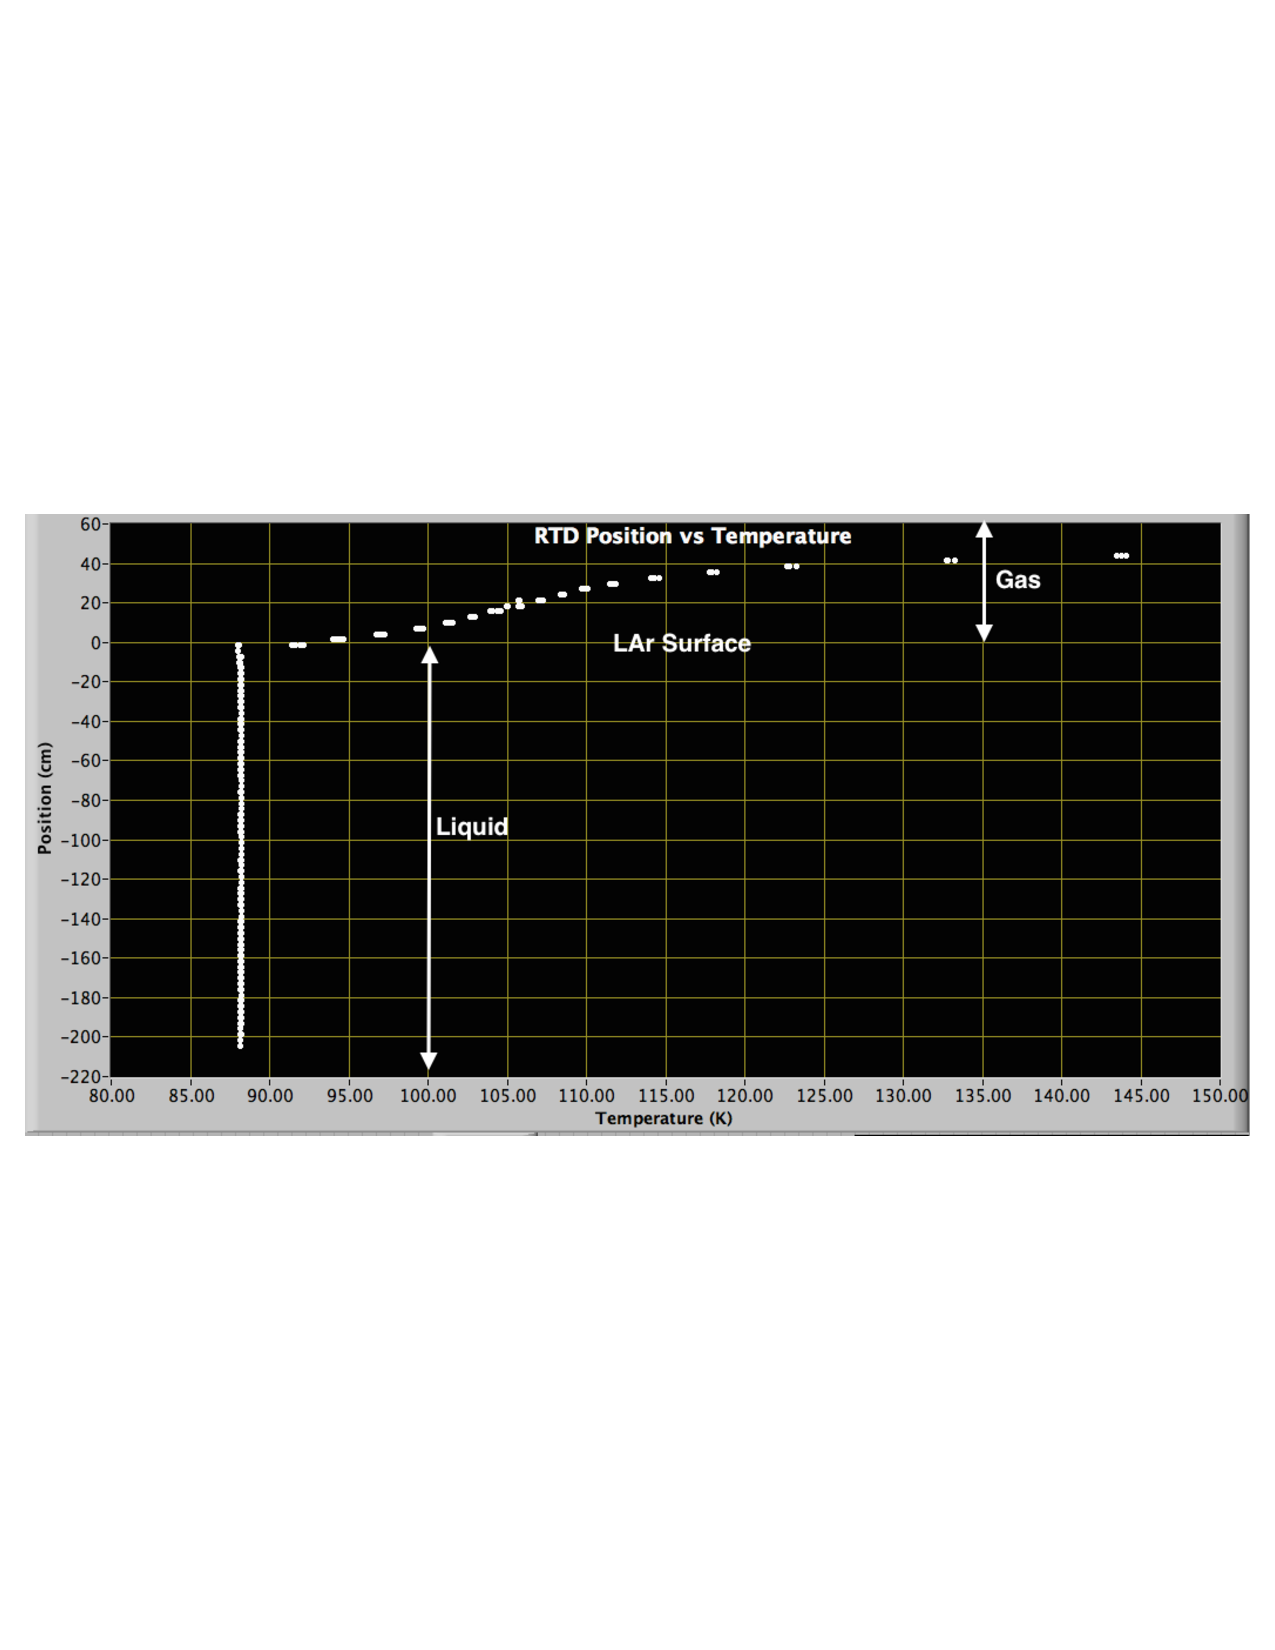
\includegraphics[width=\textwidth]{SpoolerScanFull}
\end{cdrfigure}

\subsection{Phase 1 Conclusions}

The 35T Phase 1 run has shown that the membrane cryostat technology has no innate difficulties with 
achieving the stated goals of the LBNE Conceptual Design Far Detector. Some of the 35T issues (e.g., loss 
of purity when pumps are switched) are most likely unique to the 35T. It also seems likely that in a future 
design, the pumps will be externally located, to avoid coupling acoustical vibrations into the Far Detector 
cryostat and to facilitate maintenance and repair.

%%%%%%%%%%%%%%%%%%%%%%%%%%%%

\subsection{35T Prototype Phase 2}

Phase 2 of the the 35T prototype involves installing a fully operational TPC and Photon Detector into 
the previously built cryostat.
This prototype will be filled with Liquid Argon and operated for a several-month-long Cosmic Ray run. 
External plastic scintillator paddles placed around the cryostat will be used to produce
trigger signals as well as rough position measurements of the incoming Cosmic Rays.
Commissioning is expected to begin in June 2015.
Figure~\ref{fig:tpc-35ton-trial} shows the trial assembly of the TPC outside of the cryostat. 
Figure~\ref{fig:35TTPC} shows a model of the TPC inside the cryostat.

\subsubsection{35T Phase 2 TPC Design}

\begin{cdrfigure}[35T with TPC]{35TTPC}{35T Cryostat with TPC and photon detectors installed. 
Note separate drift regions on ``near'' and ``far'' sides. 
The near side drift length is close to what is proposed for the far detector. The far
side has a shorter drift length due to lack of space.}
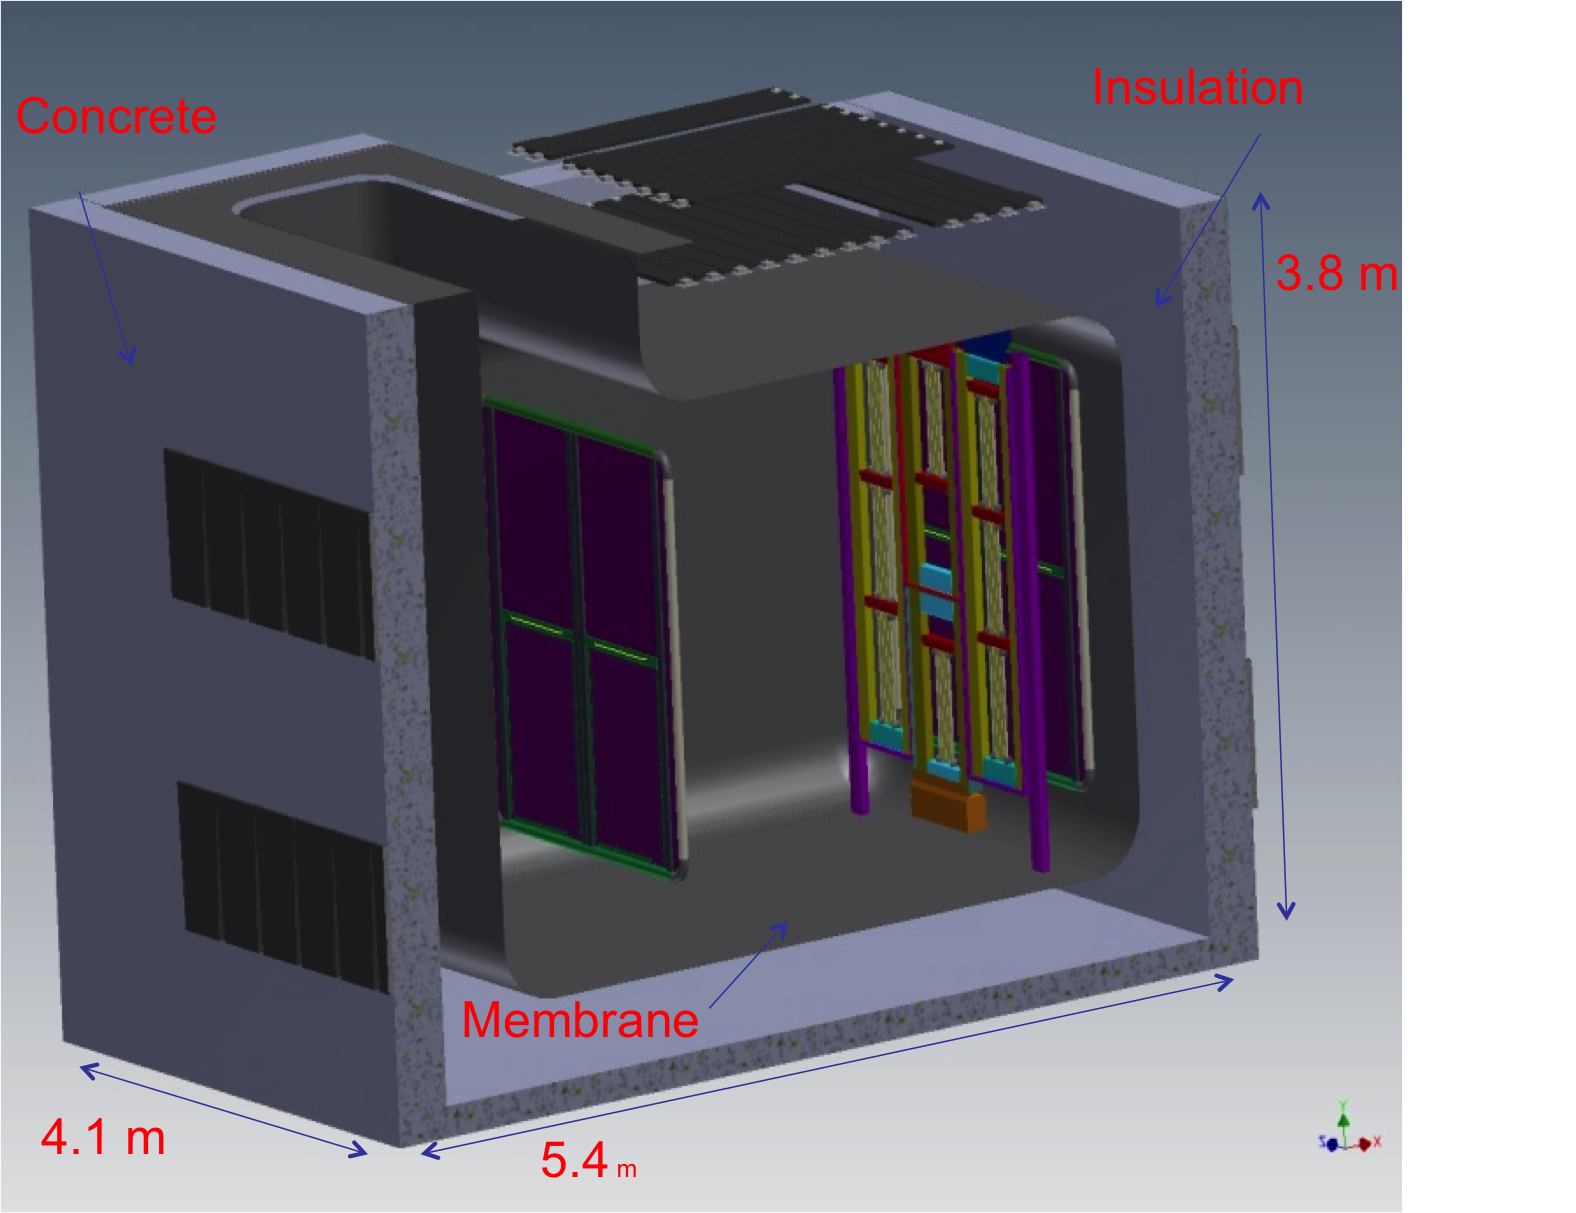
\includegraphics[height=3in]{35TTPC}  
\end{cdrfigure}

The Phase 2 prototype incorporates many of the design elements described in previous
sections of this document.
In many cases, these include novel features that have never previously been tested
in an operational TPC.
Rather than reiterate them all here, we simply tabulate some of the more important
aspects in Table~\ref{tab:35TDesign}.

\begin{cdrtable}[35T Design Aspects]{lcl}{35TDesign}{35T Design Elements}
 Design Aspect& Section & How Tested\\ \toprowrule
Modular APAs with wrapped wires & \ref{subsec:v5-tpc-chamber-apa}&Build small-scale APA Modules with FD design\\
\colhline
Vertical Gaps between APAs &\ref{subsec:v5-tpc-chamber-apa}& Assemble APAs side-by-side.\\
&&Study reco'd tracks that cross the gaps.\\
\colhline
Horizontal Gaps between APAs &\ref{subsec:v5-tpc-chamber-apa}& Build two shorter APAs and stack vertically\\
&&Study reco'd tracks that cross the gaps\\
\colhline
APAs immersed in active volume &\ref{subsec:v5-tpc-chamber-apa}& Study reco'd tracks that cross APAs\\
\colhline
Cold Digital Electronics & \ref{subsec:fe_CMOS_digital} & Measure noise performance etc. {\it in situ}\\
\colhline
Waveguide-style Photon Detector& \ref{subsec:fe_CMOS_digital}&Install in APAs. Measure lightyield\\
\colhline
Triggerless-capable DAQ & \ref{sec:daq_intro} & Take data using multiple DAQ modes\\ 
\end{cdrtable}

\subsubsection{Phase 2 Simulation, Reconstruction and Analysis}
As can be seen from Table~\ref{tab:35TDesign}, successful tests of many of the new 
design features requires simulation, reconstruction and analysis of 35T data. 
This will be done with the help of the LarSoft package, which is also used to simulate and 
reconstruct data from the ArgoNeuT and MicroBoone experiments.
Reuse of software developed for those experiments can greatly facilitate 35T development. 
However, the novel hardware features of the 35t prototype necessitate novel software developments 
as well.
Among the required new software developments are:
\begin{itemize}
\item{Code to break up the wrapped wires into as many as five individual linear segments. 
A hit on a single electronic channel can, in principle, be related to an induced signal on any of these segments.}
\item{``Disambiguation'' code to identify which of the possible wire segments was actually responsible
for the observed hit}
\item{Code for determining the start time of the event ($t_0$). Since the 35T prototype DAQ can
run ``triggerless'', methods are needed for finding the $t_0$ in data. Information from the external 
scintillator paddles as well as the internal photon detectors can be used.}
\item{Code for ``stitching''together track segments observed in different tracking volumes. 
Since hits can come from either side of the 4 APAs, there are effectively 8 separate tracking volumes, 
which are treated as separate TPCs.}
\end{itemize}

With these simulation and reconstruction tools in hand, ``physics'' analysis of the data can be undertaken.
In addition to the analyses needed to validate the new detector design elements, there are also
some analyses of basic LArTPC performance that are needed as well.
Among the highest priority analysis tasks are:

\begin{itemize}
\item{Basic detector performance: signal/noise, purity measured with tracks, track direction resolution, 
photon detector light yield}
\item{Measurement of distortions due to space charge and field non-uniformity}
\item{Measurements of different types of particles: muons, protons, neutrons, pions}
\end{itemize}

%%%%%%%%%%%%%%%%%%%%%%%%%%%%

\section{Physics Experiments with Associated Detector-Development Goals}

Two projects, ArgoNeuT and MicroBooNE,  which are physics experiments in their own right, are also contributing to the development of the LBNE experiment. Their most important role is in providing data and motivation for the development of event reconstruction and indentification software.

\subsection{ArgoNeuT - T962}
The Argon Neutrino Test (ArgoNeuT) is a 175-liter LArTPC which completed a run in the NuMI neutrino beam.  The 0.5~m $\times$ 0.5~m $\times$ 1~m LArTPC was positioned directly upstream of the MINOS near detector, which served as a muon catcher for neutrino interactions occurring in ArgoNeuT. 

ArgoNeuT began collecting data using the NuMI anti-muon neutrino beam in October 2009 and ran until  March 1, 2010.  ArgoNeuT's $\sim$10k events motivate the development of analysis tools, and are the basis for the first measurements of neutrino cross sections on argon.   An event with two $\pi^{0}$ decays is shown in Figure~\ref{fig:2pi0}.   ArgoNeuT was also the first LArTPC to be exposed to a low-energy neutrino beam and only the second worldwide to observe beam-neutrino interactions. The ArgoNeuT collaboration is currently preparing (1) a NIM paper that documents the detector performance using NuMI beam muons and (2) the first physics paper on muon-neutrino charged-current differential cross sections on argon.  See Figures~\ref{fig:ArgoNeuT_3Dreco} and~\ref{fig:ArgoNeuT-calorimetry}.

A deconvolution scheme using an FFT has been applied to the ArgoNeuT data. This procedure eliminates a problem with the ArgoNeuT electronics (which were D-Zero spares and could not be modified for ArgoNeuT). Another more significant benefit of deconvolution is that bi-polar induction-plane signals can be transformed into uni-polar collection-plane signals. An example of this is shown in Figure~\ref{fig:Argo-decon}. A selection of figures from the draft NIM paper are reproduced below.


\begin{cdrfigure}[ArgoNeuT neutrino event with four photon conversions]{2pi0}{A neutrino event with four photon conversions in the ArgoNeuT detector. The top (bottom) panel shows data from the induction (collection) plane after deconvolution.}
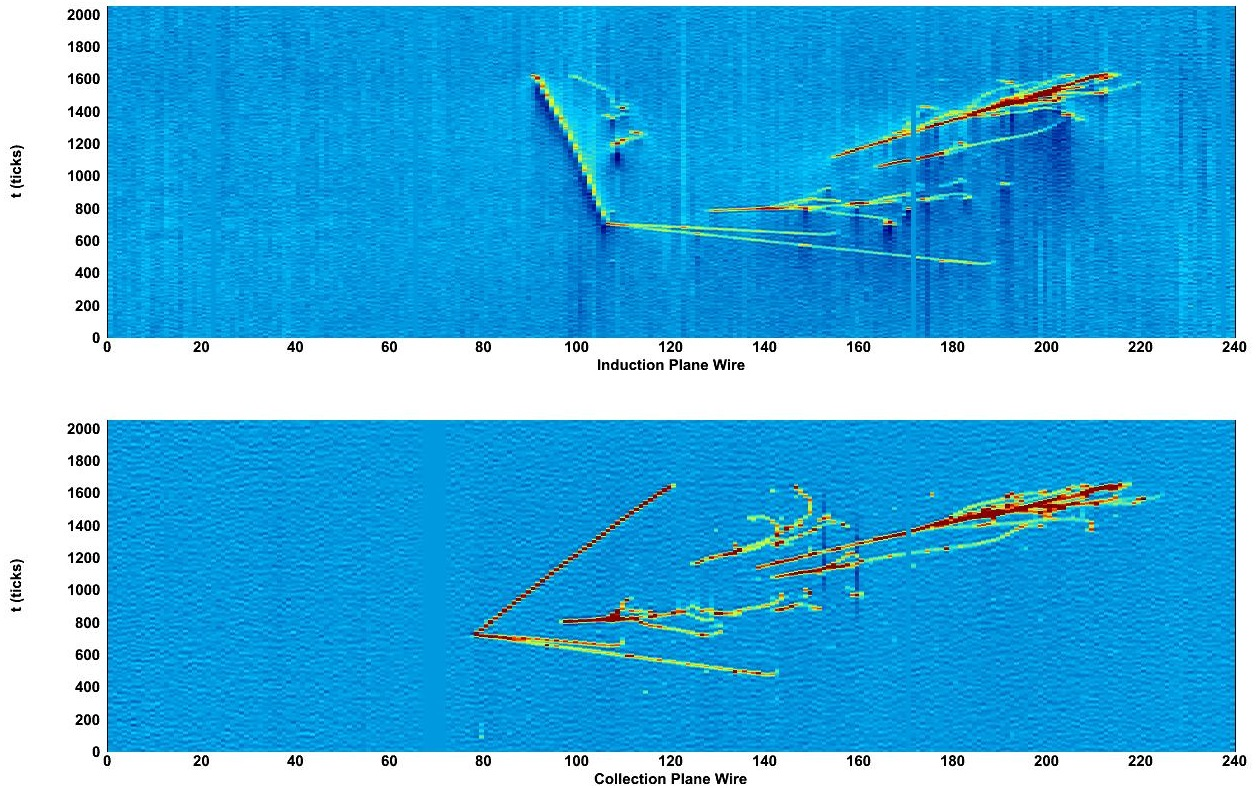
\includegraphics[width=0.7\textwidth]{ArgoNeuT_event}
\end{cdrfigure}


The applicability of ArgoNeuT is that it provides a set of data in the same range of energy as the LBNE neutrino beam, enabling the development of analysis algorithms that can be utilized for LAr-FD physics analysis with little or no modification.


\begin{cdrfigure}[Data from ArgoNeuT]{Argo-decon}{Figure from the ArgoNeuT draft NIM paper}
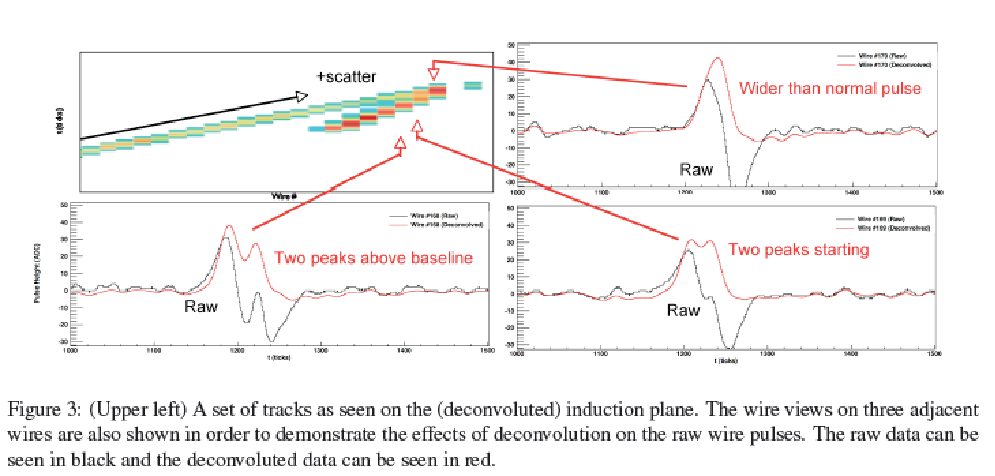
\includegraphics[width=\textwidth]{ArgoNeuT_decon}
\end{cdrfigure} %     STILL TO DO      \fixme{Can you remove the caption from the PDF and add it to this caption?}}

\begin{cdrfigure}[ArgoNeuT: status of 3D reconstruction]{ArgoNeuT_3Dreco}{Figure from the ArgoNeuT draft NIM paper showing the status of 3D reconstruction}
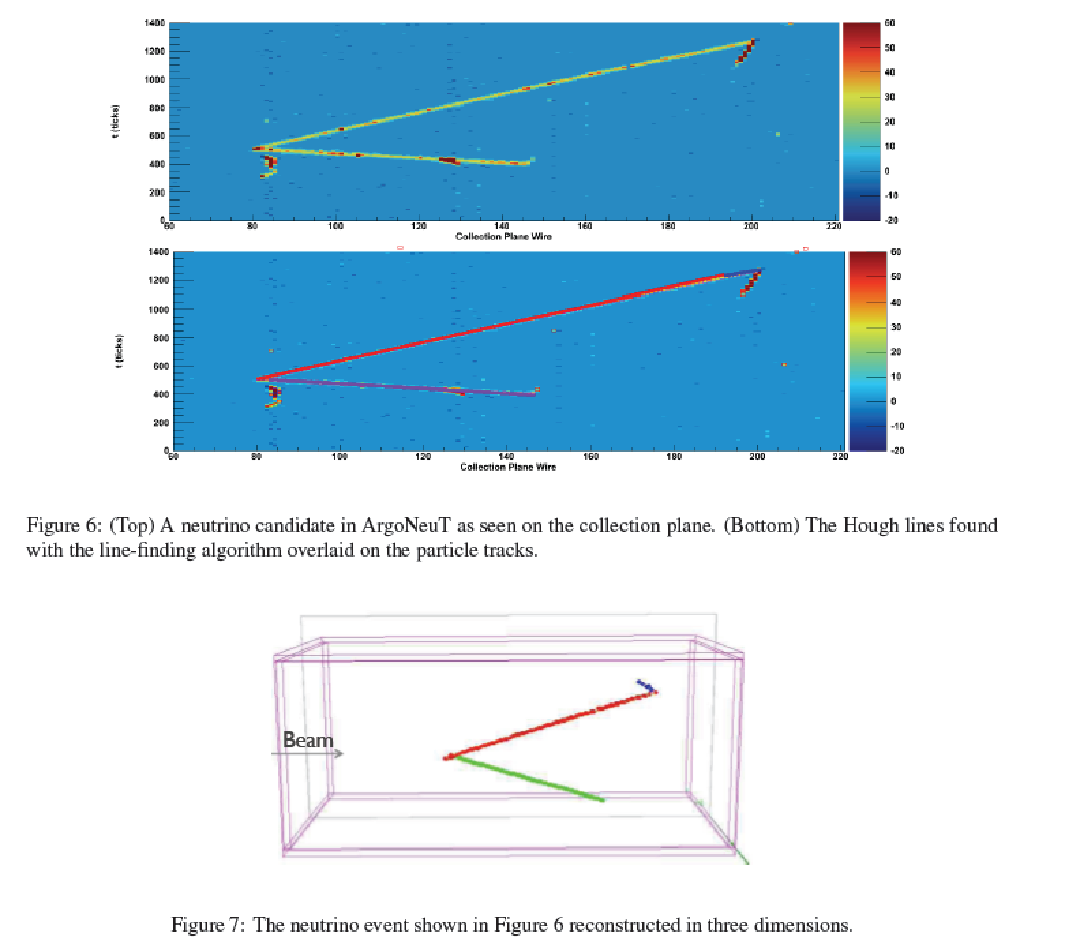
\includegraphics[width=\textwidth]{ArgoNeuT_3Dreco}
\end{cdrfigure}%     STILL TO DO       \fixme{Can you remove the caption from the PDF and add it to this caption?}}

\begin{cdrfigure}[ArgoNeuT: status of calorimetric reconstruction]{ArgoNeuT-calorimetry}{Figure from the ArgoNeuT draft NIM paper showing the status of calorimetric reconstruction.}
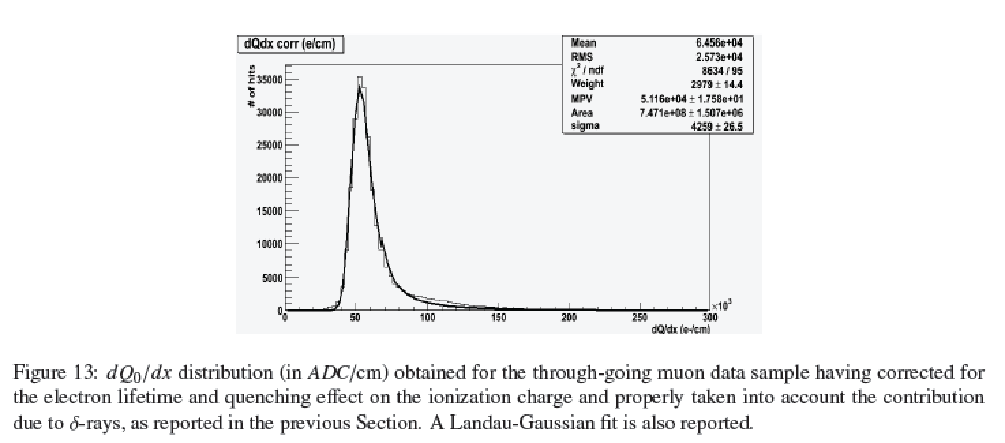
\includegraphics[width=\textwidth]{ArgoNeuT_dQdx}
\end{cdrfigure}%     STILL TO DO      \fixme{Can you remove the caption from the PDF and add it to this caption?} }

\subsection {MicroBooNE E-974}

The MicroBooNE experiment is an 89-ton active mass LArTPC, (170-ton argon mass) in the commissioning phase.  It has both a physics program and LArTPC development goals.  

MicroBooNE received stage 1 approval from the Fermilab director in 2008, partial funding through an NSF MRI in 2008 and an NSF proposal in 2009.  MicroBooNE received DOE CD-0 Mission Need in 2009, CD-1 review in 2010, CD-2/3a review in 2011, CD-3b review in 2012 and CD-4 review in December 2014. The construction of MicroBooNE experiment has been completed successfully, and detector commissioning is ongoing. It plans to start running in mid 2015. 

As well as pursuing its own physics program, MicroBooNE will collect a large sample ($\sim$100k) of low-energy neutrino events that will serve as a library for the understanding of neutrino interactions in 
LAr. Because MicroBooNE is at the surface, it will also have a large sample of cosmic rays with which it can study potential backgrounds to rare physics. The process of designing MicroBooNE has naturally stimulated several developments helpful to the LBNE program.  Studies of wire material, comparing Be-Cu with gold-plated stainless steel in terms of their electrical and mechanical properties at room and LAr temperatures, and techniques for wire-tension measurement are immediately relevant. Expertise has been developed generating simulations of electrostatic-drift fields as well as simulations of temperature and flow distributions in LAr cryostats which is being applied to the LAr-FD TPC and cryostat. MicroBooNE will use the front end of the proposed in-liquid electronics as the wire-signal amplifiers and the DAQ developed for MicroBooNE will exploit compression and data-reduction techniques to record data with 100\% livetime.

\noindent  In summary, MicroBooNE's LArTPC development goals that are pertinent to LAr-FD are
\begin{itemize}
\item large-scale testing of LBNE cryogenic front-end electronics, similar in scale to the CERN prototype
\item testing of continuous data-acquisition algorithms
\item refinement of the analysis tools developed in ArgoNeuT
\item provide costing and construction lessons-learned
\end{itemize}

\section{Summary}

Impressive progress has been made in the development of LArTPC technology over the last few years. All elements of the development program have completed the R\&D phase. Credible conceptual designs exist for all systems in LAr-FD. The technical activities described in this chapter are properly characterized as preliminary engineering design.

The most significant deficiency is the lack of fully-automated event reconstruction. Algorithms have been developed within the LAr community and are being successfully applied to ArgoNeuT data as well as to simulated MicroBooNE data. The algorithms have individually shown that the high efficiency and excellent background rejection capabilities of an LArTPC are achievable. The task remains to combine them into a single package. 


